%%%%%%%%%%%%%%%%%%%%%%%%%%%%%%%%%%%%%%%%%%%%%%%%%%%%%%%%%%%
% LG-CARL bilingual experiment report
% Chinese version first, English version second.
%%%%%%%%%%%%%%%%%%%%%%%%%%%%%%%%%%%%%%%%%%%%%%%%%%%%%%%%%%%

\documentclass[9pt,a4paper,twocolumn,twoside]{rho-class/rho}
\usepackage[english]{babel}
\usepackage{CJKutf8}
\usepackage{amsmath}

%----------------------------------------------------------
% Title
%----------------------------------------------------------

\doctype{Research Article}
\title{LG-CARL: Line-Graph Congestion-Aware Reinforcement Learning for Adaptive Routing}

%----------------------------------------------------------
% Authors, Affiliations and dates
%----------------------------------------------------------

\author[a,1]{Xiangyi Liu}
\affil[a]{Course Project in Computer Networks and Machine Learning}
\dates{Compiled on \today}

%----------------------------------------------------------
% Corresponding author and document information
%----------------------------------------------------------

\corres{Contact: \href{mailto:lnubruni@gmail.com}{lnubruni@gmail.com}.}
\docinfo{This report documents a runnable implementation of LG-CARL, including the simulator, GNN-DQN routing agent, baseline policies, quantitative evaluation, and route replay visualizations. The report is organized with the Chinese version first and the English version second.}

\journalname{LG-CARL}
\journal{Adaptive Routing Report}
\theday{\today}
\vol{1}
\no{1}

%----------------------------------------------------------
% Abstract and Keywords
%----------------------------------------------------------

\begin{abstract}
This report presents LG-CARL, a congestion-aware adaptive routing system that combines directed line-graph representation learning with deep reinforcement learning. The project models each directed network link as a node in a line graph, applies a GraphSAGE-style encoder to link-level state features, and uses a DQN agent to select among candidate end-to-end paths for each traffic demand. The implementation includes a lightweight network simulator, synthetic and real-topology experiments, baseline policies, training and evaluation scripts, and route replay visualizations. Experiments show that LG-CARL learns stable routing behavior and performs close to shortest-path and dynamic-shortest-path routing under regular traffic, while the heavy-congestion scenario remains challenging and exposes directions for future reward and training improvements.
\end{abstract}

\keywords{Adaptive routing, line graph, graph neural network, DQN, congestion-aware routing, network simulation}

\begin{document}

\maketitle
\thispagestyle{firststyle}

%==========================================================
% Chinese version
%==========================================================

\begin{CJK*}{UTF8}{gbsn}

\section*{中文版本}
\addcontentsline{toc}{section}{中文版本}

\section*{摘要}
\addcontentsline{toc}{section}{摘要}

本文介绍 LG-CARL，一个结合 directed line graph、GraphSAGE 和 DQN 的拥塞感知自适应路由实验系统。系统将每条有向链路建模为 line graph 中的节点，使用 GNN 编码链路级状态，并通过 DQN 在候选端到端路径中选择路由。实验表明，在常规流量场景下，LG-CARL 能够学习到接近 shortest path 和 dynamic shortest path 的路由行为；在强拥塞场景下，模型虽然比随机路由更好，并表现出更强的负载均衡倾向，但在时延、丢包和吞吐方面仍落后于 dynamic shortest path。该结果说明项目实现完整且具有解释价值，同时也暴露出 reward 设计和拥塞训练设置仍需改进。

\textbf{关键词：} 自适应路由；链路图；图神经网络；DQN；拥塞感知；网络仿真。

\section{引言}

\rhostart{L}G-CARL 是一个面向计算机网络动态路由问题的实验系统。传统最短路算法主要依据静态链路代价进行选路，在网络负载变化、队列积压和链路拥塞出现时，单纯依赖静态距离并不一定能得到低时延或低丢包的路径。本项目将路由问题建模为强化学习任务：环境不断产生流量请求，智能体根据当前链路状态在若干候选路径中选择一条路由，并通过时延、丢包、拥塞和路径切换等反馈学习策略。

本项目的核心思想是将原始网络拓扑转换为 directed line graph。原图中的一条有向链路在 line graph 中成为一个节点；如果两条有向链路可以连续转发，则在 line graph 中连接它们。这样，GNN 的消息传递发生在链路状态之间，而不是只发生在路由器节点之间。由于拥塞本质上更接近链路级现象，例如链路利用率、队列长度、丢包率和链路延迟，因此 line graph 表示更适合表达路由决策所需的动态状态。

项目目标不是证明模型在所有场景下都优于传统启发式方法，而是实现一个完整、可运行、可解释的 GNN + RL 路由实验框架。该框架包括网络仿真器、候选路径生成、Line-Graph GraphSAGE 编码器、path-level DQN、baseline 对比、实验结果表格和可视化 GIF。

\subsection*{贡献}
\addcontentsline{toc}{subsection}{贡献}

本文主要贡献如下：

\begin{itemize}
    \item 提出并实现一个以链路为中心的自适应路由实验系统，将 directed line graph 表示、GraphSAGE 编码器和 DQN 路径选择结合起来。
    \item 构建轻量网络仿真器，能够模拟链路负载、队列、利用率、时延、丢包和服务衰减过程。
    \item 提供 Random-K、Shortest Path 和 Dynamic Shortest Path baseline，用于定量比较学习式路由策略。
    \item 在 NSFNet-like 拓扑和 SNDlib Polska 真实拓扑上进行常规流量和拥塞流量实验，并给出可视化 replay 分析。
\end{itemize}

\section{相关工作}

\subsection{传统路由与流量工程}

早期互联网路由协议主要依赖分布式控制和静态或半静态链路代价。RIP \cite{hedrick1988rip} 和 OSPF \cite{moy1998ospf} 代表了经典的距离向量和链路状态路由协议，ECMP \cite{hopps2000ecmp} 进一步通过等价路径分摊流量。MPLS \cite{rosen2001mpls} 和 RSVP-TE \cite{awduche2001rsvp} 则为显式路径控制和流量工程提供了协议基础。这些机制稳定、可解释且工程成熟，但通常需要人工配置权重或策略，对快速变化的负载和拥塞状态适应能力有限。

为了提升网络资源利用率，流量工程研究开始从单纯最短路转向全局优化。Fortz 和 Thorup 研究了通过优化 OSPF 权重实现 Internet traffic engineering \cite{fortz2000internet,fortz2002traffic}；Applegate 等研究了在流量矩阵变化和不确定性下的鲁棒 intra-domain routing \cite{appelgate2003making}；Roughan 等对骨干网流量变化进行了测量建模 \cite{roughan2002experience}；Kandula 等进一步讨论了响应性和稳定性之间的权衡 \cite{kandula2005walking}。这些工作说明路由优化不仅要考虑最短路径，还要考虑负载均衡、鲁棒性和稳定性。

SDN 进一步将路由控制从分布式协议推向集中式、可编程控制。OpenFlow \cite{mckeown2008openflow}、DevoFlow \cite{curtis2011devoflow}、Hedera \cite{alfares2010hedera}、Google B4 \cite{jain2013b4} 和 SWAN \cite{hong2013swan} 展示了集中式控制在数据中心和广域网中的潜力。Kreutz 等 \cite{kreutz2015sdn} 和 Akyildiz 等 \cite{akyildiz2014roadmap} 对 SDN 架构和流量工程进行了系统综述。与这些优化和控制平面工作相比，LG-CARL 关注的是在一个可控仿真环境中学习候选路径选择策略，并通过 reward 将拥塞、丢包和稳定性纳入统一目标。

\subsection{强化学习路由与学习式网络控制}

强化学习为动态路由提供了一种无需显式解析模型的自适应优化思路。Q-learning \cite{watkins1992qlearning} 和现代强化学习框架 \cite{sutton2018reinforcement} 为此类方法奠定了理论基础。Boyan 和 Littman 的 Q-routing \cite{boyan1993packet} 是较早将强化学习用于动态网络路由的代表性工作；Ant-based routing \cite{schoonderwoerd1996ant,dicaro1998antnet} 则从群体智能角度探索了自适应路径选择。深度学习兴起后，DQN \cite{mnih2015human}、Double DQN \cite{vanhasselt2016deep}、Prioritized Experience Replay \cite{schaul2016prioritized} 和 Dueling Network \cite{wang2016dueling} 使基于值函数的控制能够处理更复杂的状态空间。

学习式网络控制也被用于资源管理、拥塞控制、视频传输和流量工程。DeepRM \cite{mao2016resource} 通过深度强化学习学习资源调度；Pensieve \cite{mao2017neural} 将 RL 用于自适应码率控制；Aurora \cite{jay2019deep} 和 Classic Meets Modern \cite{abbasloo2020classic} 探索了学习式拥塞控制；Valadarsky 等 \cite{valadarsky2017learning} 和 Xu 等 \cite{xu2018experience} 则讨论了深度强化学习在路由和网络控制中的应用。与这些工作相比，本项目使用强化学习学习 path-level 选择，但强调 line graph 表示，使链路级拥塞状态成为策略输入的核心。

\subsection{图神经网络与网络建模}

图神经网络为处理拓扑结构数据提供了通用工具。Scarselli 等 \cite{scarselli2009gnn} 提出了早期 GNN 框架，随后 GCN \cite{kipf2017semi}、GraphSAGE \cite{hamilton2017inductive}、GAT \cite{velickovic2018graph}、MPNN \cite{gilmer2017mpnn} 和 GIN \cite{xu2019powerful} 推动了图表示学习的发展。Battaglia 等 \cite{battaglia2018relational} 从 relational inductive bias 角度总结了 graph networks 的表达能力。这些工作共同说明，当问题天然具有图结构时，显式利用拓扑关系通常比普通 MLP 更有归纳偏置。

通信网络是 GNN 的自然应用场景。RouteNet \cite{rusek2020routenet} 证明 GNN 可以建模拓扑、路由和流量之间的关系，并预测 delay、jitter 和 loss 等网络 KPI。RouteNet-Fermi \cite{suarezvarela2022routenetfermi} 进一步提升了网络性能建模能力。Suarez-Varela 等 \cite{suarezvarela2022graph} 系统总结了 GNN 在通信网络中的应用场景和机会；IGNNITION \cite{pujolperich2021ignnition} 则试图降低网络系统中构建 GNN 原型的门槛。Almasan 等 \cite{almasan2019deep} 将 GNN 与 DRL agent 结合，用于提升路由优化在不同拓扑上的泛化能力；Abrol 等 \cite{abrol2024deep} 使用 DGCNN 和 DQN 进行自适应流量路由。这些研究与 LG-CARL 最为接近，但本项目采用 directed line graph，使 GNN 的节点直接对应链路而非路由器，从而更强调链路拥塞状态的传播建模。

\subsection{与本工作的关系}

综上，传统流量工程提供了强 baseline 和可解释优化目标，强化学习提供了动态决策框架，GNN 提供了拓扑泛化和结构表示能力。LG-CARL 将这三条线索结合：用 line graph 表示链路级状态，用 GraphSAGE 学习链路嵌入，用 DQN 在候选路径集合上进行决策。与完全端到端的黑盒路由不同，本项目保留了 k-shortest candidate paths，使动作空间可控且便于可视化解释；与传统 shortest path 相比，它能够将拥塞、丢包和切换稳定性纳入学习目标。

\section{方法}

\subsection{网络状态建模}

原始网络被表示为有向图 $G=(V,E)$，其中 $V$ 是路由器集合，$E$ 是有向链路集合。每条链路 $e=(u,v)$ 具有容量、基础延迟、当前负载、队列长度、利用率、丢包率和故障状态等属性。

为了更直接地建模链路之间的拥塞传播关系，项目构建 directed line graph $G_L=(V_L,E_L)$。其中 $V_L$ 中的每个节点对应原图中的一条有向链路。如果 $e_1=(u,v)$ 与 $e_2=(v,w)$ 可以连续转发，则在 line graph 中加入边 $e_1 \rightarrow e_2$。该设计使 GNN 能够在相邻链路之间聚合信息，从而学习局部拥塞模式。

\subsection{候选路径动作空间}

每一步环境产生一个流量请求：

\begin{equation}
f_t=(s_t,d_t,b_t),
\end{equation}

其中 $s_t$ 是源节点，$d_t$ 是目的节点，$b_t$ 是需求大小。系统首先通过 k-shortest paths 生成 $K$ 条候选路径：

\begin{equation}
\mathcal{P}_{s,d}=\{p_1,p_2,\ldots,p_K\}.
\end{equation}

智能体并不是在所有可能路径中任意搜索，而是在有限候选路径中评分和选择。这种设计降低了动作空间复杂度，同时保证候选路径本身具有基本可行性。

\subsection{Path-Level DQN}

模型先使用 GraphSAGE 风格的 line-graph 编码器得到每条链路的嵌入表示。对某条候选路径 $p_k$，模型聚合路径上所有链路嵌入，并拼接路径特征、源节点嵌入、目的节点嵌入和需求大小，最后通过 MLP 输出该路径的 Q 值：

\begin{equation}
Q(s_t,p_k)=\mathrm{MLP}\left(h(p_k),x(p_k),e_s,e_d,b_t\right).
\end{equation}

评估阶段选择 Q 值最高的有效候选路径：

\begin{equation}
p^*=\arg\max_{p_k \in \mathcal{P}_{s,d}} Q(s_t,p_k).
\end{equation}

\subsection{奖励函数}

奖励函数采用负代价形式，主要惩罚以下因素：路径时延、丢包、最大链路利用率、路径切换代价、关键链路风险和非法动作。概念上可以写为：

\begin{equation}
r_t=-\left(
\alpha D_t+\beta L_t+\gamma U_t+\lambda S_t+\eta R_t
\right),
\end{equation}

其中 $D_t$ 表示归一化时延，$L_t$ 表示丢包，$U_t$ 表示最大链路利用率，$S_t$ 表示路径切换代价，$R_t$ 表示关键链路风险。由于 reward 是负代价，所以数值越接近 0 表示越好。

\section{实现}

项目使用 Python、PyTorch 和 NetworkX 实现。主要模块包括：

\begin{itemize}
    \item \textbf{Routing environment}: 负责生成流量请求、维护网络状态、执行路由动作并返回 reward。
    \item \textbf{Network simulator}: 维护链路 load、queue、utilization、delay 和 loss。
    \item \textbf{Line graph utilities}: 将原始拓扑转换为 directed line graph，并生成链路特征。
    \item \textbf{DQN agent}: 使用 replay buffer、target network 和 epsilon-greedy 策略进行训练。
    \item \textbf{Baselines}: 包括 Random-K、Shortest Path 和 Dynamic Shortest Path。
    \item \textbf{Visualization}: 输出训练曲线、评估柱状图、拓扑图和 route replay GIF。
\end{itemize}

\begin{figure}[H]
    \centering
    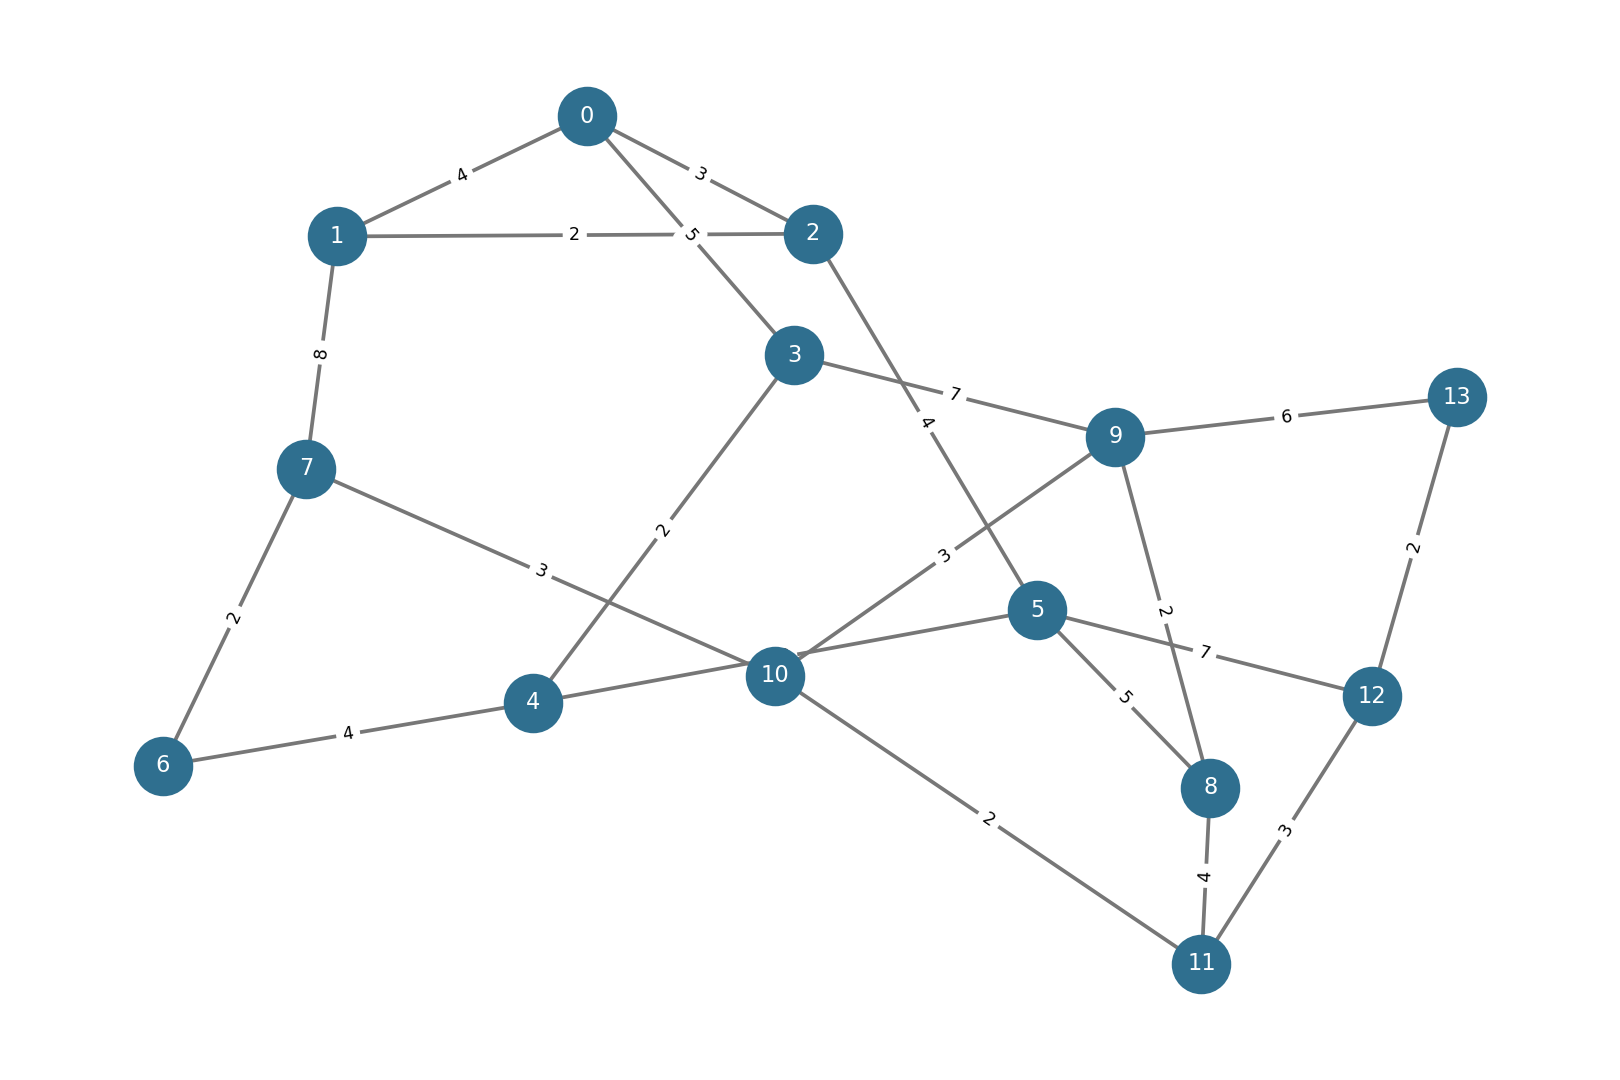
\includegraphics[width=0.95\columnwidth]{figures/topology.png}
    \caption{NSFNet-like topology used by the default experiment.}
    \label{fig:cn_topology}
\end{figure}

\section{实验设置}

实验覆盖三类主要配置。第一类是默认 NSFNet-like 拓扑，使用合成 uniform traffic；第二类是 SNDlib Polska 真实拓扑和归一化 demand matrix；第三类是更高需求、更慢服务率的 SNDlib Polska congested 配置，用作拥塞压力测试。

评价指标包括：

\begin{itemize}
    \item \textbf{Average delay}: 每一步路由后的平均路径时延，越低越好。
    \item \textbf{Loss rate}: 丢弃流量占总需求的比例，越低越好。
    \item \textbf{Throughput}: 每一步平均成功交付的流量，越高越好。
    \item \textbf{Max utilization}: episode 中最大链路利用率，越低通常表示瓶颈压力越小。
    \item \textbf{Load balance std}: 链路利用率标准差，越低表示负载分布越均衡。
    \item \textbf{Switch rate}: 路径切换比例，用于衡量路由稳定性。
\end{itemize}

\section{实验结果}

\begin{table*}[t]
    \caption{Selected evaluation results. Lower delay/loss/utilization is better; higher throughput is better.}
    \label{tab:cn_results}
    \centering
    \begin{tabular}{llrrrrr}
        \toprule
        \textbf{Scenario} & \textbf{Method} & \textbf{Avg Delay} & \textbf{Loss} & \textbf{Throughput} & \textbf{Max Util.} & \textbf{Balance Std} \\
        \midrule
        NSFNet uniform & Shortest Path & 9.778 & 0.000 & 5.467 & 0.217 & 0.0196 \\
        NSFNet uniform & Dynamic Shortest & 9.777 & 0.000 & 5.467 & 0.217 & 0.0196 \\
        NSFNet uniform & LG-CARL & 10.880 & 0.000 & 5.467 & 0.193 & 0.0205 \\
        SNDlib Polska regular & Shortest Path & 4.512 & 0.000 & 5.709 & 0.167 & 0.0154 \\
        SNDlib Polska regular & Dynamic Shortest & 4.512 & 0.000 & 5.709 & 0.167 & 0.0154 \\
        SNDlib Polska regular & LG-CARL & 4.517 & 0.000 & 5.709 & 0.167 & 0.0153 \\
        SNDlib Polska congested & Shortest Path & 464.048 & 0.561 & 25.737 & 1.500 & 0.6123 \\
        SNDlib Polska congested & Dynamic Shortest & 439.005 & 0.617 & 22.454 & 1.500 & 0.4835 \\
        SNDlib Polska congested & LG-CARL & 699.294 & 0.726 & 16.060 & 1.500 & 0.2976 \\
        \bottomrule
    \end{tabular}
\end{table*}

从 \tabref{tab:cn_results} 可以看到，在默认 NSFNet uniform 场景中，LG-CARL 的平均时延为 10.880，高于 dynamic shortest path 的 9.777，但最大链路利用率从 0.217 降至 0.193，说明模型倾向于一定程度上分散链路负载。在 SNDlib Polska regular 场景中，LG-CARL 的平均时延 4.517 与 shortest path 的 4.512 几乎相同，loss rate 也保持为 0，说明常规负载下模型可以学习到接近强 baseline 的行为。

在 congested 场景中，LG-CARL 相比 random routing 有明显改善，但仍落后于 dynamic shortest path。其平均时延为 699.294，高于 dynamic shortest path 的 439.005；loss rate 为 0.726，也高于 shortest path 的 0.561。与此同时，LG-CARL 的 load balance std 为 0.2976，低于 shortest path 和 dynamic shortest path，说明模型确实更均匀地分散了负载，但这种分散没有转化为更低的丢包和更高的吞吐。

\begin{figure*}[t]
    \centering
    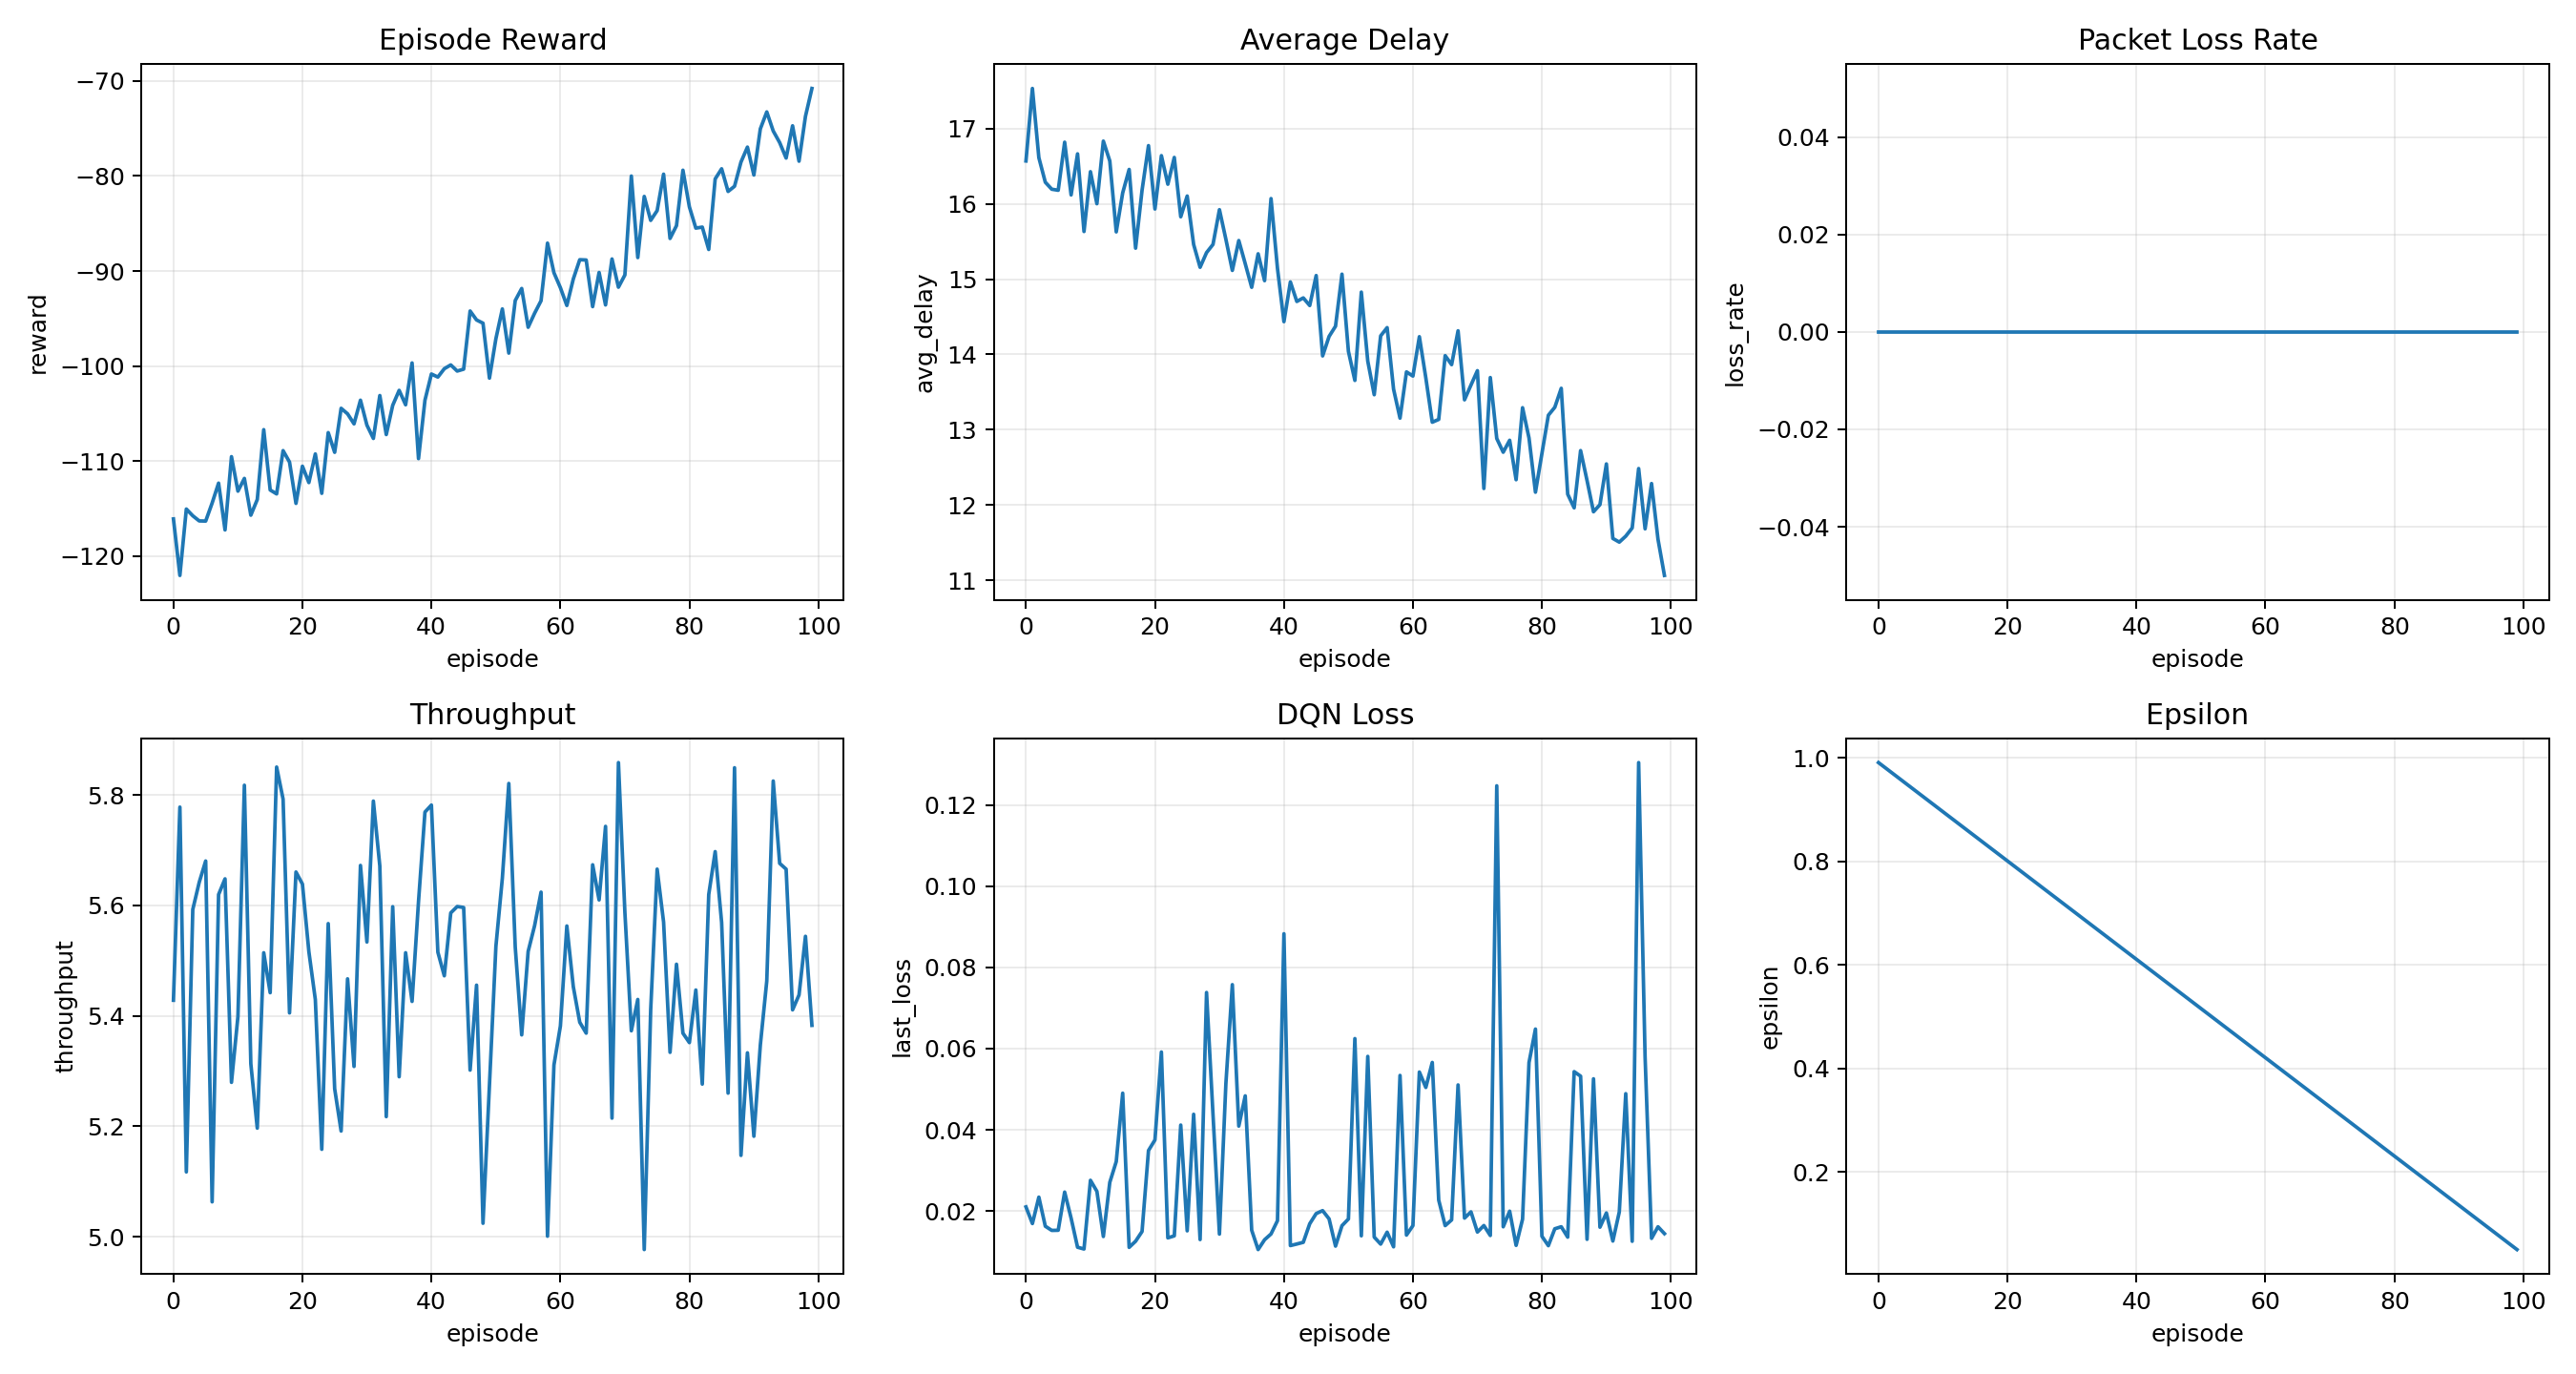
\includegraphics[width=0.92\textwidth]{figures/training_curves.png}
    \caption{Training curves for reward, average delay, packet loss rate, throughput, DQN loss, and epsilon.}
    \label{fig:cn_training}
\end{figure*}

\begin{figure*}[t]
    \centering
    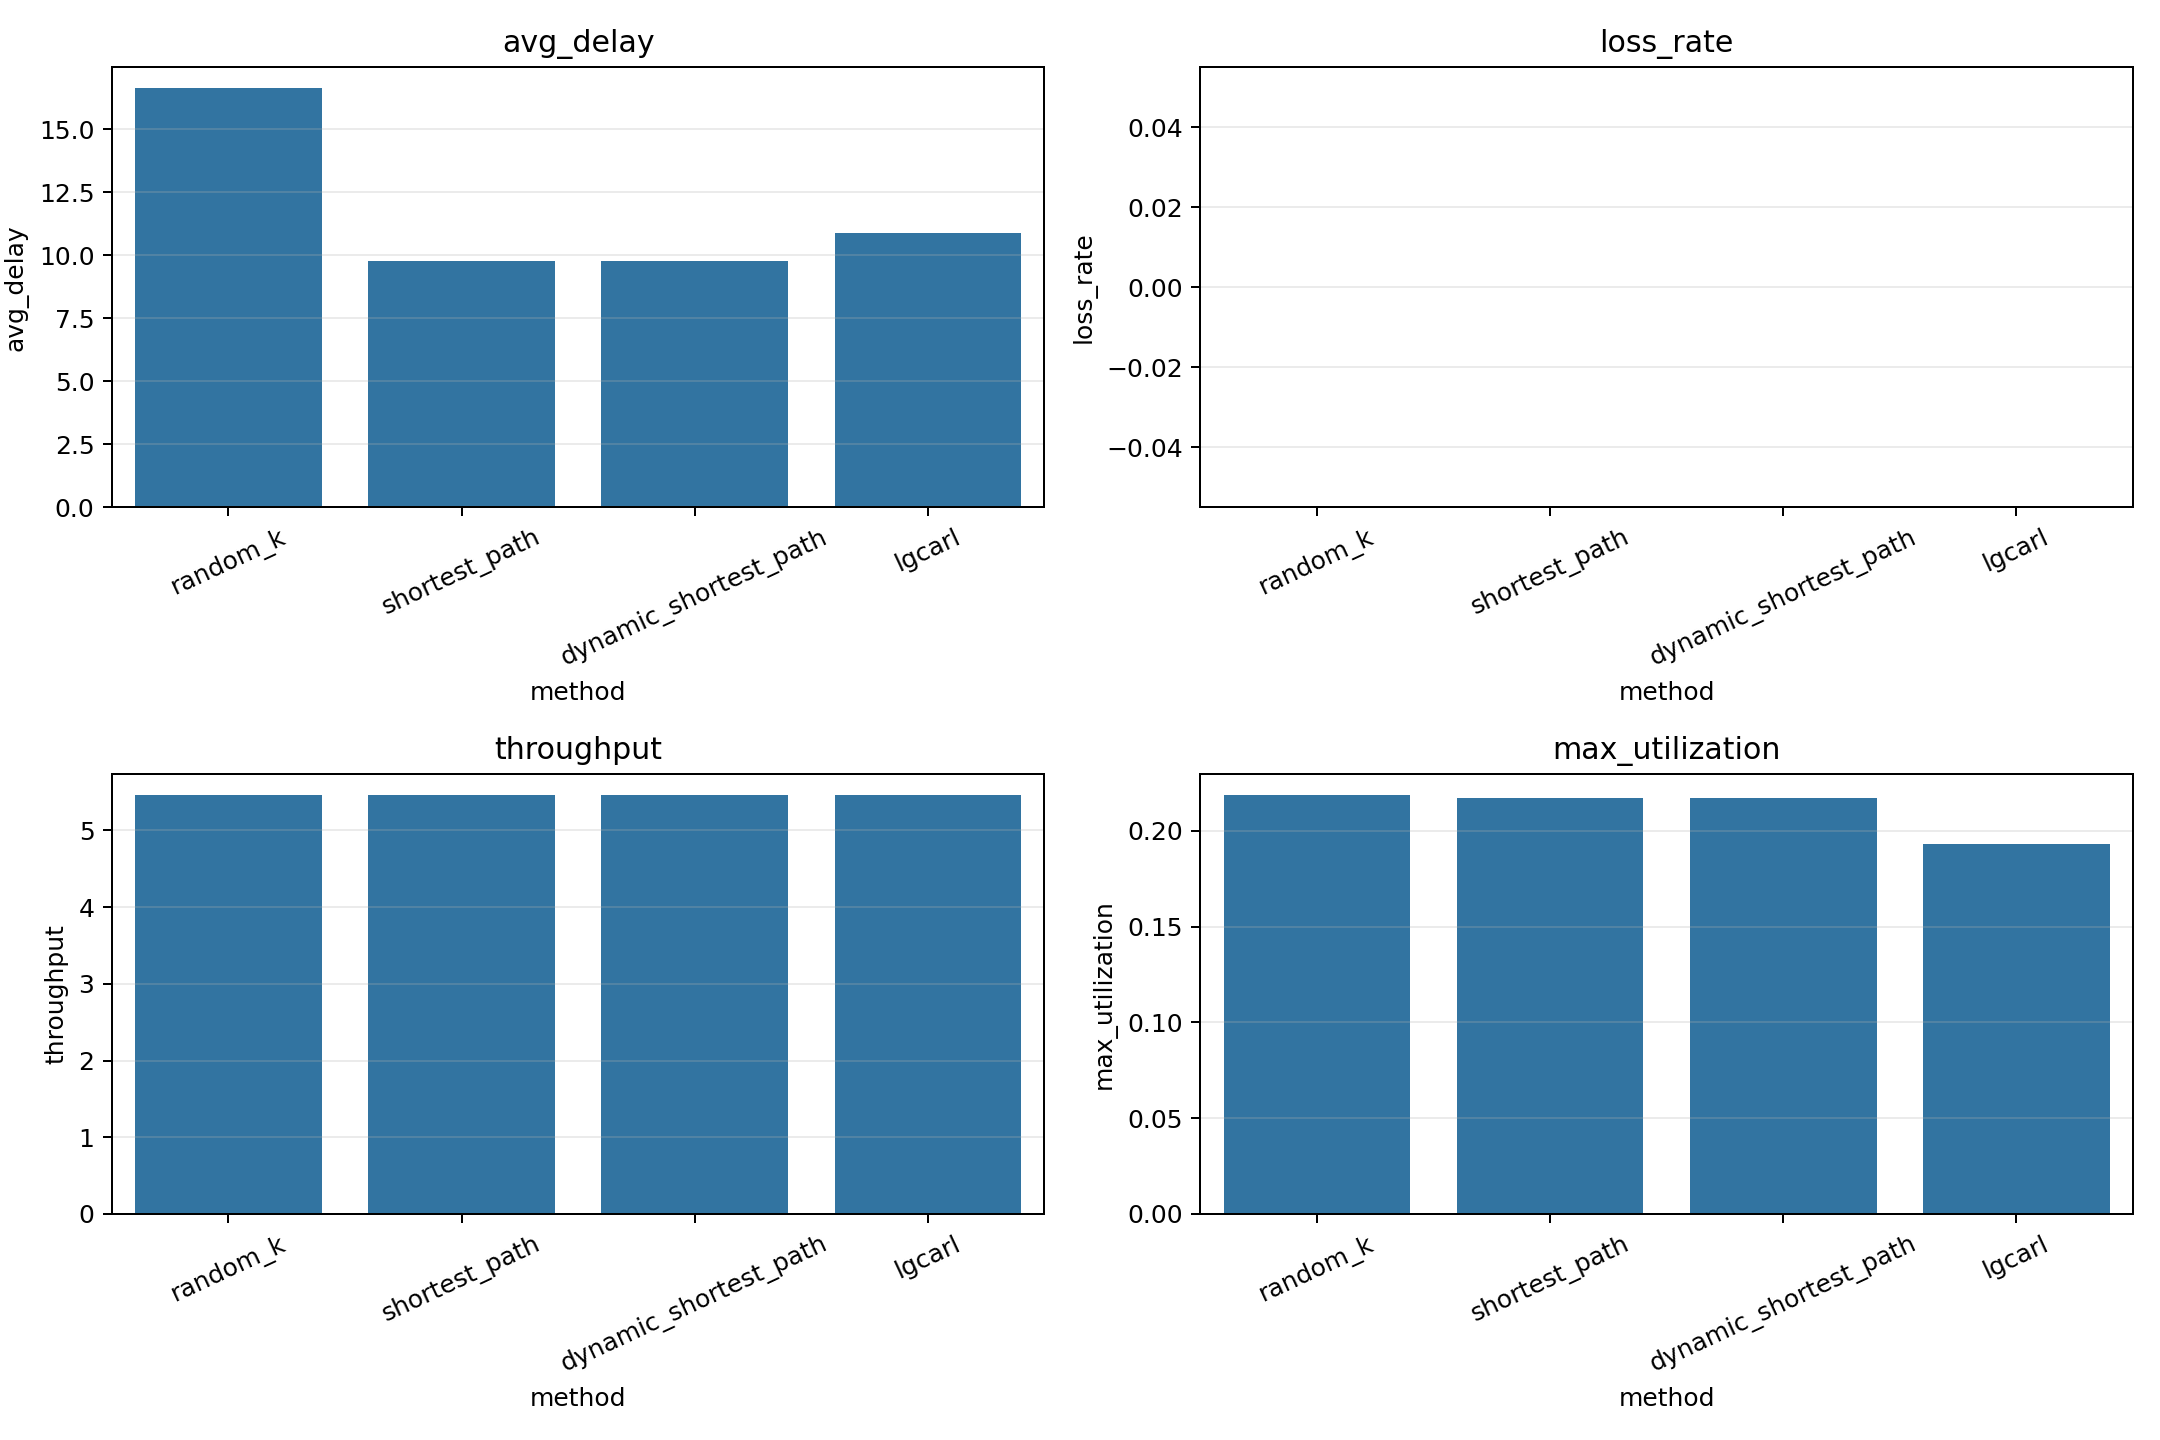
\includegraphics[width=0.92\textwidth]{figures/eval_bars.png}
    \caption{Evaluation bar charts comparing LG-CARL with routing baselines.}
    \label{fig:cn_eval}
\end{figure*}

\section{可视化分析}

为了让模型行为更容易解释，项目实现了 route replay 可视化。图中节点表示路由器，边表示链路；边颜色越接近红色表示链路利用率越高；蓝白色高亮线表示 LG-CARL 当前选择的路径。右侧面板显示当前 flow、demand、delay、loss、delivered traffic 和 max utilization。

\begin{figure}[H]
    \centering
    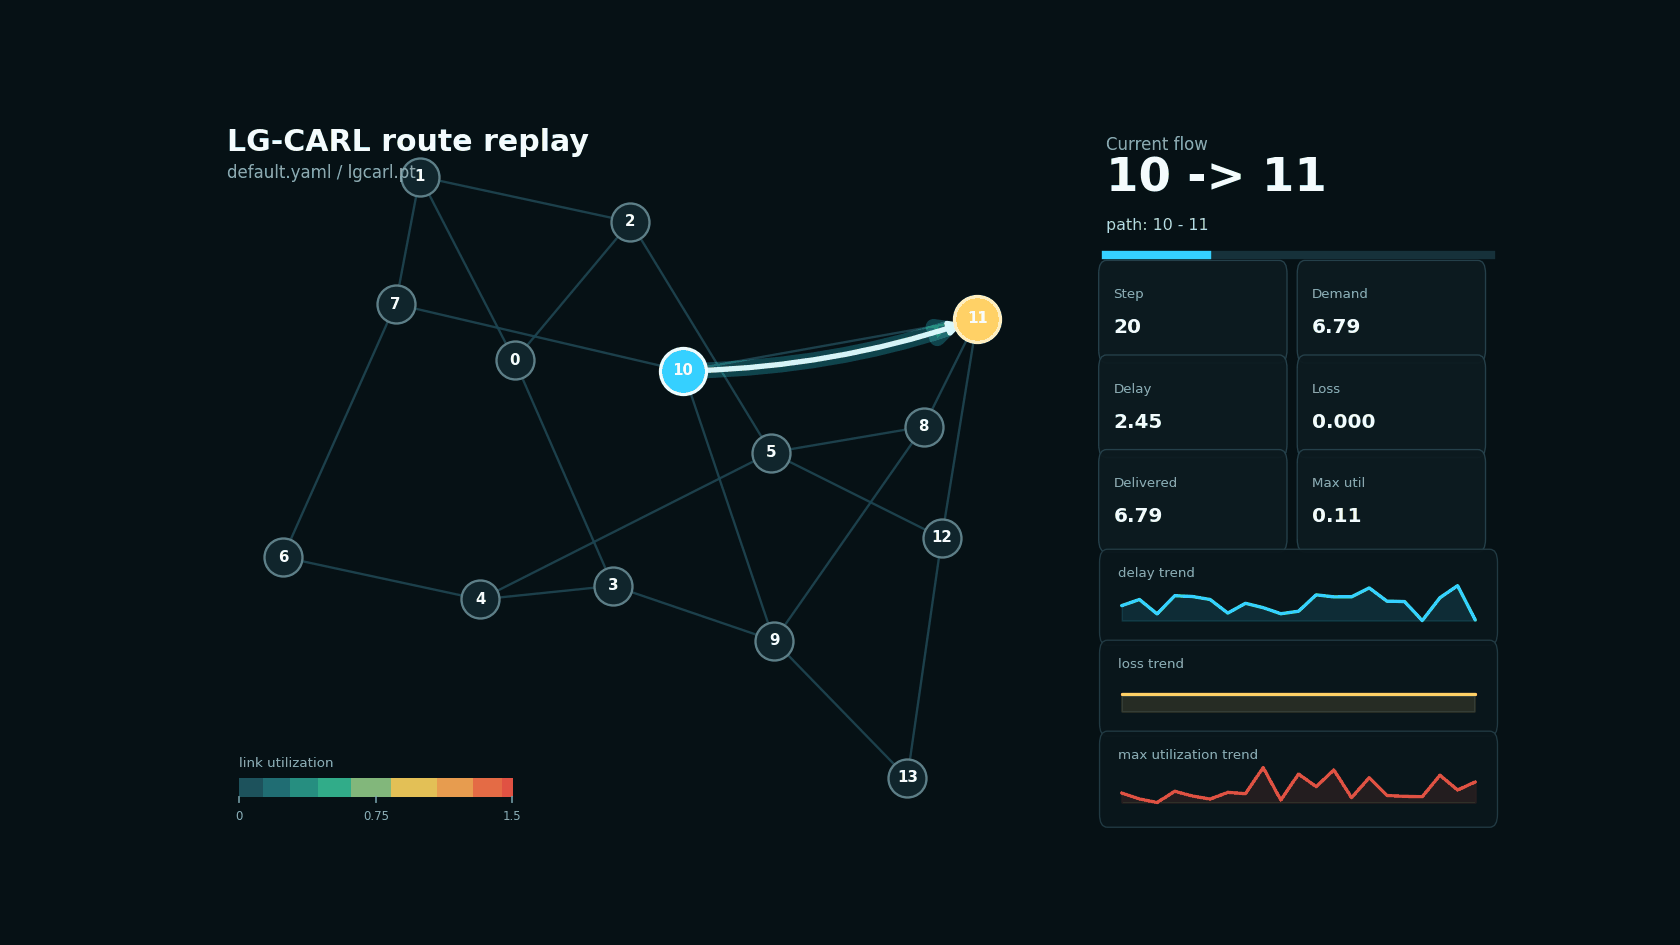
\includegraphics[width=0.98\columnwidth]{figures/route_replay_normal_frame.png}
    \caption{Route replay frame under regular traffic. The selected path is highlighted in cyan.}
    \label{fig:cn_replay_regular}
\end{figure}

\begin{figure}[H]
    \centering
    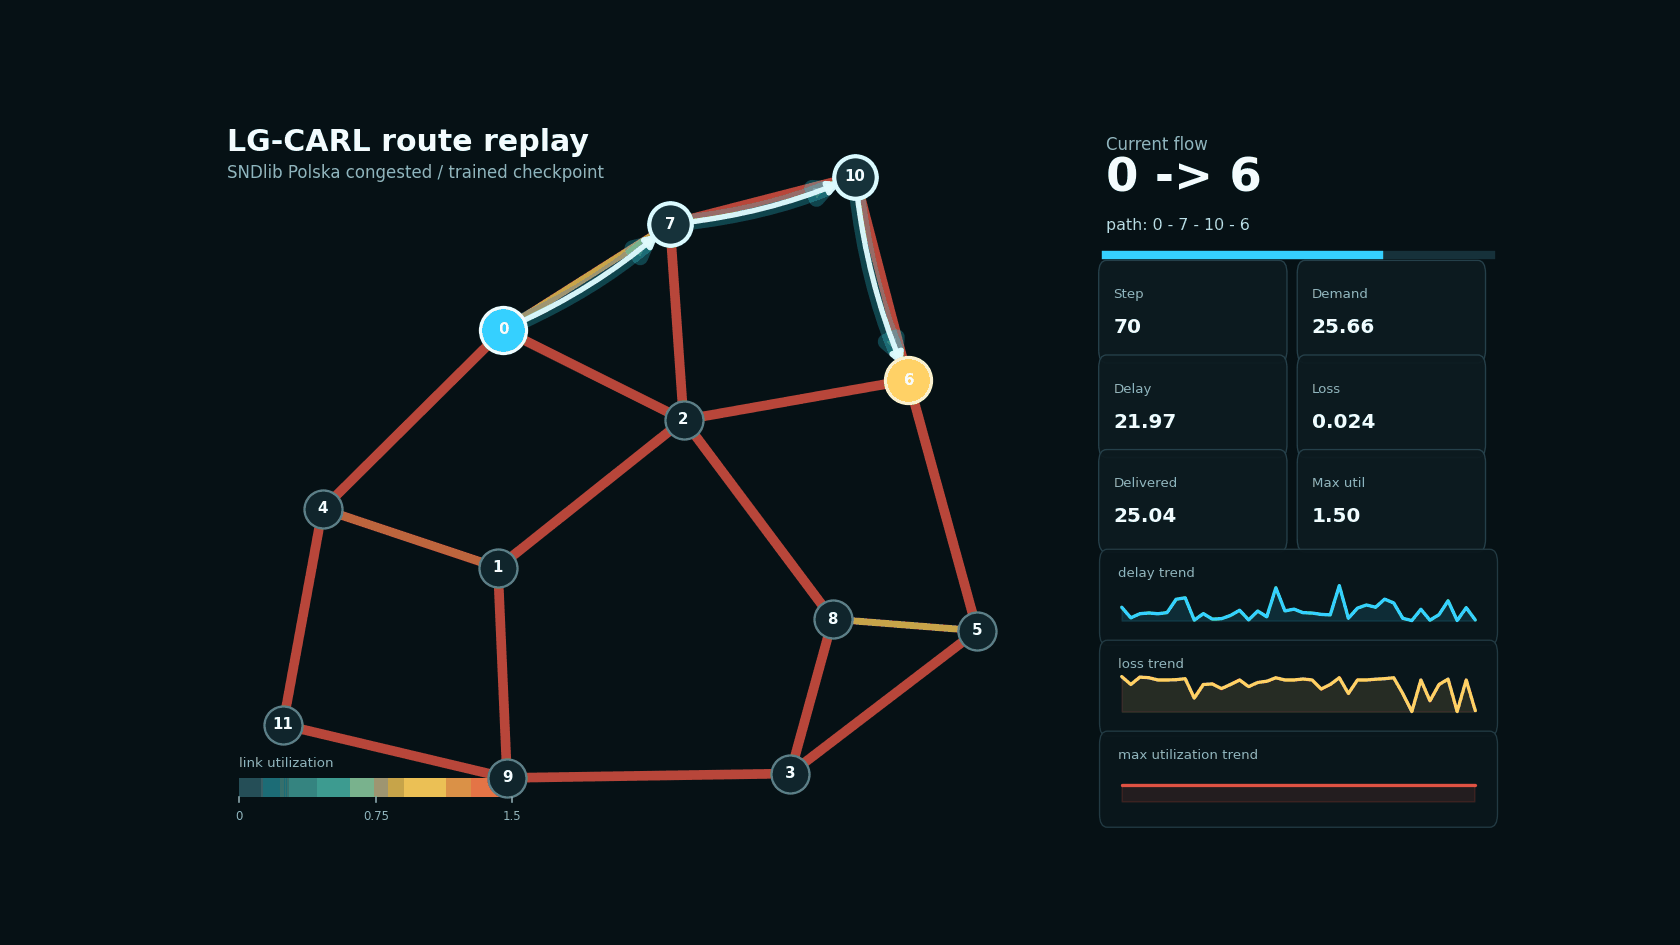
\includegraphics[width=0.98\columnwidth]{figures/route_replay_congested_frame.png}
    \caption{Route replay frame under heavy congestion. Many links become orange or red, and packet loss appears.}
    \label{fig:cn_replay_congested}
\end{figure}

常规场景中，大部分链路保持冷色，loss 基本为 0。拥塞场景中，多条链路达到高利用率，max utilization 经常顶到 1.5，并且 loss trend 出现波动。这说明 GIF 更适合用于解释模型行为和网络状态变化，而不是单独证明模型优于 baseline。最终性能仍应以 \tabref{tab:cn_results} 中的定量指标为准。

\section{结论}

本项目完成了一个可运行的 GNN + RL 自适应路由实验系统。LG-CARL 能够将链路级状态编码到 directed line graph 中，并通过 DQN 在候选路径中选择路由。在常规流量下，模型能达到接近 shortest path 和 dynamic shortest path 的性能；在部分指标上，例如最大链路利用率或负载均衡，它表现出分散负载的倾向。

然而，在强拥塞场景下，当前策略尚未超过 dynamic shortest path。实验结果表明，模型虽然学习到了负载均衡行为，但该行为没有充分转化为更低的丢包率和更高的吞吐量。这说明 reward 权重、训练稳定性、拥塞数据分布和强化学习算法仍有进一步优化空间。

总体而言，LG-CARL 作为课程项目是完整的：它包含明确的问题建模、可运行代码、多 baseline 对比、真实拓扑支持、定量分析和可视化解释。未来可以继续加入 reward ablation、double DQN、多随机种子置信区间和未见拓扑泛化实验。

\end{CJK*}

\clearpage
\setcounter{section}{0}
\setcounter{figure}{0}
\setcounter{table}{0}

%==========================================================
% English version
%==========================================================

\section*{English Version}
\addcontentsline{toc}{section}{English Version}

\section*{Abstract}
\addcontentsline{toc}{section}{Abstract}

This report presents LG-CARL, a congestion-aware adaptive routing system that combines directed line graphs, GraphSAGE, and DQN. The system models each directed link as a node in a line graph, uses a GNN to encode link-level states, and applies a DQN policy to select among candidate end-to-end paths. Experiments show that LG-CARL learns behavior close to shortest-path and dynamic-shortest-path routing under regular traffic. Under heavy congestion, it improves over random routing and shows stronger load-balancing behavior, but it still underperforms dynamic shortest path in delay, loss, and throughput. The result demonstrates a complete and interpretable implementation while exposing reward design and congestion training as important future directions.

\textbf{Keywords:} adaptive routing; line graph; graph neural network; DQN; congestion-aware routing; network simulation.

\section{Introduction}

\rhostart{L}G-CARL is an experimental system for adaptive routing in computer networks. Classical shortest-path routing mainly relies on static link costs. When network load changes dynamically, queues grow, and bottleneck links become congested, the shortest static path may no longer provide low delay or low packet loss. This project formulates routing as a reinforcement learning problem: the environment generates traffic demands, the agent selects one route from several candidate paths, and the selected action is evaluated through delay, loss, congestion, and switching-related feedback.

The key idea of this project is to represent the network as a directed line graph. In the original graph, routers are nodes and directed links are edges. In the line graph, each directed link becomes a node. If two directed links can be used consecutively for forwarding, an edge is created between their corresponding line-graph nodes. This makes message passing occur between link states rather than only between router nodes. Since congestion is primarily a link-level phenomenon, this representation is suitable for modeling utilization, queue length, loss rate, and link delay.

The goal of the project is not to claim that the learned policy dominates all routing heuristics in every setting. Instead, it aims to provide a complete, runnable, and interpretable GNN + RL routing framework. The framework includes a network simulator, candidate path generation, a Line-Graph GraphSAGE encoder, a path-level DQN agent, baseline comparisons, quantitative tables, and route replay visualizations.

\subsection*{Contributions}
\addcontentsline{toc}{subsection}{Contributions}

The main contributions are:

\begin{itemize}
    \item We implement a link-centric adaptive routing system that combines directed line-graph representation, a GraphSAGE encoder, and DQN-based path selection.
    \item We build a lightweight simulator that updates link load, queue, utilization, delay, loss, and service decay.
    \item We include Random-K, Shortest Path, and Dynamic Shortest Path baselines for quantitative comparison.
    \item We evaluate the system on an NSFNet-like topology and the SNDlib Polska topology under both regular and congested traffic, with route replay visualizations for interpretation.
\end{itemize}

\section{Related Work}

\subsection{Classical Routing and Traffic Engineering}

Early Internet routing protocols rely on distributed control and static or semi-static link costs. RIP \cite{hedrick1988rip} and OSPF \cite{moy1998ospf} are representative distance-vector and link-state protocols, while ECMP \cite{hopps2000ecmp} distributes traffic over equal-cost paths. MPLS \cite{rosen2001mpls} and RSVP-TE \cite{awduche2001rsvp} provide protocol-level support for explicit path control and traffic engineering. These mechanisms are stable, interpretable, and mature, but they often require manually configured weights or policies and may adapt slowly to rapidly changing load.

Traffic engineering research moved beyond pure shortest-path routing toward global optimization. Fortz and Thorup studied OSPF weight optimization for Internet traffic engineering \cite{fortz2000internet,fortz2002traffic}. Applegate et al. investigated robust intra-domain routing under changing and uncertain traffic matrices \cite{appelgate2003making}. Roughan et al. measured and modeled backbone traffic variability \cite{roughan2002experience}, and Kandula et al. studied the trade-off between responsiveness and stability \cite{kandula2005walking}. These works show that routing optimization must account for load balancing, robustness, and stability, not merely path length.

Software-defined networking further pushed routing control toward centralized and programmable systems. OpenFlow \cite{mckeown2008openflow}, DevoFlow \cite{curtis2011devoflow}, Hedera \cite{alfares2010hedera}, Google B4 \cite{jain2013b4}, and SWAN \cite{hong2013swan} demonstrate the potential of centralized control in data-center and wide-area networks. Kreutz et al. \cite{kreutz2015sdn} and Akyildiz et al. \cite{akyildiz2014roadmap} provide broader surveys of SDN architectures and traffic engineering. Compared with these optimization and control-plane systems, LG-CARL focuses on learning a candidate-path selection policy in a controllable simulator, using reward terms to combine congestion, loss, and routing stability.

\subsection{Reinforcement Learning for Routing and Network Control}

Reinforcement learning provides an adaptive optimization framework that does not require a fully specified analytic model of the network. Q-learning \cite{watkins1992qlearning} and the general RL framework \cite{sutton2018reinforcement} form the foundation for such methods. Q-routing by Boyan and Littman \cite{boyan1993packet} is one of the earliest examples of reinforcement learning for dynamic packet routing. Ant-based routing \cite{schoonderwoerd1996ant,dicaro1998antnet} explored adaptive path selection from a swarm-intelligence perspective. With deep learning, DQN \cite{mnih2015human}, Double DQN \cite{vanhasselt2016deep}, Prioritized Experience Replay \cite{schaul2016prioritized}, and Dueling Networks \cite{wang2016dueling} made value-based control more suitable for high-dimensional states.

Learning-based network control has also been applied to resource management, congestion control, adaptive video streaming, and traffic engineering. DeepRM \cite{mao2016resource} uses deep reinforcement learning for resource scheduling. Pensieve \cite{mao2017neural} applies RL to adaptive bitrate streaming. Aurora \cite{jay2019deep} and Classic Meets Modern \cite{abbasloo2020classic} explore learning-based congestion control. Valadarsky et al. \cite{valadarsky2017learning} and Xu et al. \cite{xu2018experience} discuss deep reinforcement learning for routing and network control. LG-CARL follows this learning-based direction but emphasizes line-graph state representation, making link-level congestion the central policy input.

\subsection{Graph Neural Networks and Network Modeling}

Graph neural networks provide a general framework for learning from topological data. Scarselli et al. \cite{scarselli2009gnn} introduced an early GNN formulation. Later models such as GCN \cite{kipf2017semi}, GraphSAGE \cite{hamilton2017inductive}, GAT \cite{velickovic2018graph}, MPNN \cite{gilmer2017mpnn}, and GIN \cite{xu2019powerful} advanced graph representation learning. Battaglia et al. \cite{battaglia2018relational} summarized graph networks from the perspective of relational inductive bias. These works show that when a problem is naturally graph-structured, explicitly exploiting topology can provide a useful inductive bias compared with plain MLPs.

Communication networks are a natural application domain for GNNs. RouteNet \cite{rusek2020routenet} showed that GNNs can model the relationship among topology, routing, and traffic and predict network KPIs such as delay, jitter, and loss. RouteNet-Fermi \cite{suarezvarela2022routenetfermi} further improved GNN-based network performance modeling. Suarez-Varela et al. \cite{suarezvarela2022graph} surveyed opportunities for GNNs in communication networks, and IGNNITION \cite{pujolperich2021ignnition} lowered the barrier to prototyping GNNs for networking systems. Almasan et al. \cite{almasan2019deep} combined GNNs with a DRL agent to improve routing optimization across different topologies, while Abrol et al. \cite{abrol2024deep} used DGCNN and DQN for adaptive traffic routing. LG-CARL is closest to this line of work, but it uses a directed line graph so that GNN nodes directly correspond to links rather than routers, emphasizing link-level congestion propagation.

\subsection{Position of This Work}

Overall, classical traffic engineering provides strong baselines and interpretable objectives, reinforcement learning provides a dynamic decision-making framework, and GNNs provide topology-aware representation learning. LG-CARL combines these directions: it represents link-level state with a line graph, learns link embeddings with GraphSAGE, and uses DQN to select among candidate paths. Unlike fully black-box routing, it preserves k-shortest candidate paths, keeping the action space controlled and visualizable. Unlike pure shortest-path routing, it can include congestion, loss, and switching stability in the learning objective.

\section{Method}

\subsection{Network State Modeling}

The physical network is represented as a directed graph $G=(V,E)$, where $V$ is the set of routers and $E$ is the set of directed links. Each link $e=(u,v)$ has capacity, base delay, current load, queue length, utilization, loss rate, and failure state.

To model congestion propagation between adjacent links, the project constructs a directed line graph $G_L=(V_L,E_L)$. Each node in $V_L$ corresponds to one directed link in the original graph. If $e_1=(u,v)$ and $e_2=(v,w)$ can be used consecutively in a forwarding path, the line graph contains the edge $e_1 \rightarrow e_2$. This allows the GNN to aggregate information across adjacent links and learn local congestion patterns.

\subsection{Candidate Path Action Space}

At each step, the environment generates a traffic demand:

\begin{equation}
f_t=(s_t,d_t,b_t),
\end{equation}

where $s_t$ is the source node, $d_t$ is the destination node, and $b_t$ is the demand size. The system first generates $K$ candidate paths using k-shortest paths:

\begin{equation}
\mathcal{P}_{s,d}=\{p_1,p_2,\ldots,p_K\}.
\end{equation}

The agent does not search over all possible paths. It scores and selects from a bounded set of feasible candidate paths. This design reduces the action-space complexity while keeping the selected action interpretable as an end-to-end route.

\subsection{Path-Level DQN}

The model first applies a GraphSAGE-style encoder on the directed line graph to produce link embeddings. For each candidate path $p_k$, the model aggregates the embeddings of the links on that path and concatenates path-level features, source and destination embeddings, and the demand size. A multilayer perceptron then outputs a Q-value for the candidate path:

\begin{equation}
Q(s_t,p_k)=\mathrm{MLP}\left(h(p_k),x(p_k),e_s,e_d,b_t\right).
\end{equation}

During evaluation, the policy selects the valid candidate path with the largest Q-value:

\begin{equation}
p^*=\arg\max_{p_k \in \mathcal{P}_{s,d}} Q(s_t,p_k).
\end{equation}

\subsection{Reward Function}

The reward is implemented as a negative cost. The agent is penalized for high path delay, packet loss, high maximum link utilization, frequent route switching, critical-link risk, and invalid actions. Conceptually:

\begin{equation}
r_t=-\left(
\alpha D_t+\beta L_t+\gamma U_t+\lambda S_t+\eta R_t
\right),
\end{equation}

where $D_t$ is normalized delay, $L_t$ is packet loss, $U_t$ is maximum link utilization, $S_t$ is switching cost, and $R_t$ is critical-link risk. Since reward is a negative cost, values closer to zero are better.

\section{Implementation}

The project is implemented in Python with PyTorch and NetworkX. The main modules are:

\begin{itemize}
    \item \textbf{Routing environment}: generates traffic demands, maintains network state, executes routing actions, and returns rewards.
    \item \textbf{Network simulator}: updates link load, queue, utilization, delay, and loss.
    \item \textbf{Line graph utilities}: convert the original topology into a directed line graph and build link features.
    \item \textbf{DQN agent}: uses replay buffer, target network, and epsilon-greedy exploration.
    \item \textbf{Baselines}: include Random-K, Shortest Path, and Dynamic Shortest Path.
    \item \textbf{Visualization}: generates training curves, evaluation bars, topology plots, and route replay GIFs.
\end{itemize}

\begin{figure}[H]
    \centering
    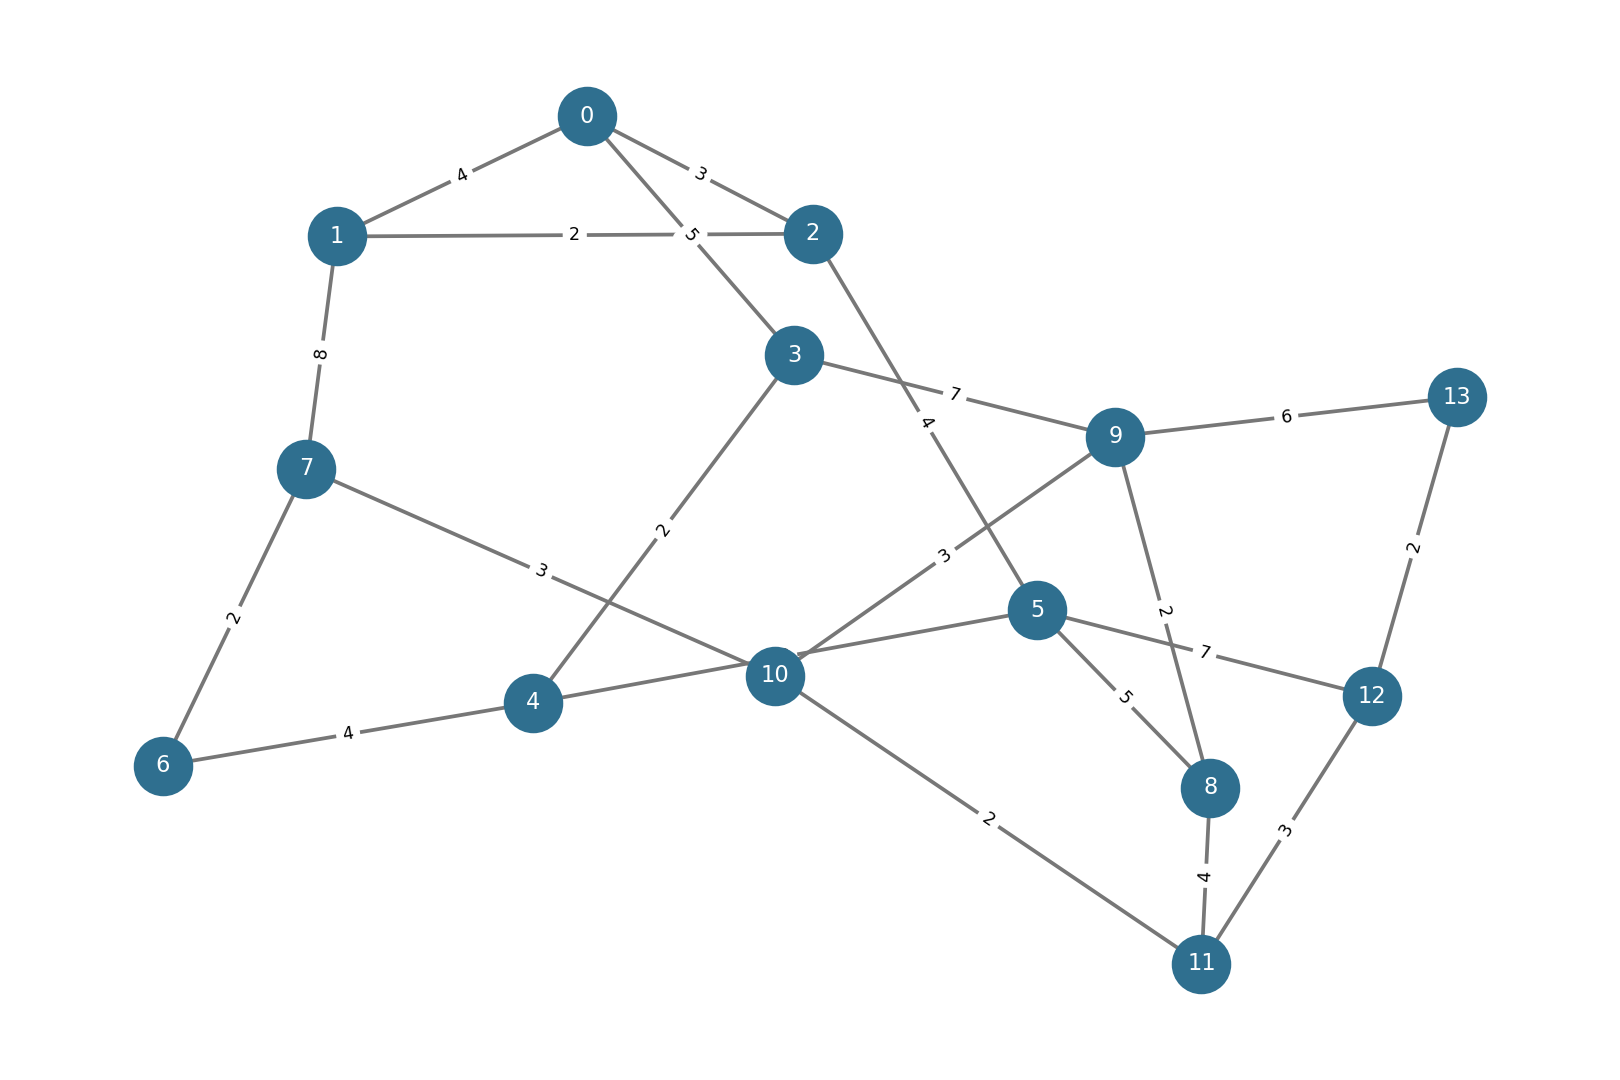
\includegraphics[width=0.95\columnwidth]{figures/topology.png}
    \caption{NSFNet-like topology used by the default experiment.}
    \label{fig:en_topology}
\end{figure}

\section{Experimental Setup}

The experiments cover three major configurations. The first one uses an NSFNet-like topology with synthetic uniform traffic. The second one uses the SNDlib Polska topology with a normalized real demand matrix. The third one uses a congested SNDlib Polska configuration with larger demands and slower service, serving as a stress test.

The evaluation metrics are:

\begin{itemize}
    \item \textbf{Average delay}: mean path delay after routing, lower is better.
    \item \textbf{Loss rate}: dropped traffic divided by total demand, lower is better.
    \item \textbf{Throughput}: average delivered traffic per step, higher is better.
    \item \textbf{Max utilization}: maximum link utilization within an episode, lower usually indicates less bottleneck pressure.
    \item \textbf{Load balance std}: standard deviation of link utilization, lower means more balanced traffic distribution.
    \item \textbf{Switch rate}: fraction of steps that change a route for the same source-destination pair.
\end{itemize}

\section{Results}

\begin{table*}[t]
    \caption{Selected evaluation results. Lower delay/loss/utilization is better; higher throughput is better.}
    \label{tab:en_results}
    \centering
    \begin{tabular}{llrrrrr}
        \toprule
        \textbf{Scenario} & \textbf{Method} & \textbf{Avg Delay} & \textbf{Loss} & \textbf{Throughput} & \textbf{Max Util.} & \textbf{Balance Std} \\
        \midrule
        NSFNet uniform & Shortest Path & 9.778 & 0.000 & 5.467 & 0.217 & 0.0196 \\
        NSFNet uniform & Dynamic Shortest & 9.777 & 0.000 & 5.467 & 0.217 & 0.0196 \\
        NSFNet uniform & LG-CARL & 10.880 & 0.000 & 5.467 & 0.193 & 0.0205 \\
        SNDlib Polska regular & Shortest Path & 4.512 & 0.000 & 5.709 & 0.167 & 0.0154 \\
        SNDlib Polska regular & Dynamic Shortest & 4.512 & 0.000 & 5.709 & 0.167 & 0.0154 \\
        SNDlib Polska regular & LG-CARL & 4.517 & 0.000 & 5.709 & 0.167 & 0.0153 \\
        SNDlib Polska congested & Shortest Path & 464.048 & 0.561 & 25.737 & 1.500 & 0.6123 \\
        SNDlib Polska congested & Dynamic Shortest & 439.005 & 0.617 & 22.454 & 1.500 & 0.4835 \\
        SNDlib Polska congested & LG-CARL & 699.294 & 0.726 & 16.060 & 1.500 & 0.2976 \\
        \bottomrule
    \end{tabular}
\end{table*}

As shown in \tabref{tab:en_results}, LG-CARL obtains an average delay of 10.880 in the NSFNet uniform setting, compared with 9.777 for dynamic shortest path. However, its maximum utilization is lower, decreasing from 0.217 to 0.193, which suggests that the learned policy tends to distribute traffic more broadly. In the SNDlib Polska regular setting, LG-CARL obtains an average delay of 4.517, nearly identical to the 4.512 achieved by shortest-path routing, while maintaining zero loss. This indicates that the model can learn behavior close to strong baselines under regular load.

In the congested setting, LG-CARL improves over random routing but still underperforms dynamic shortest path. Its average delay is 699.294, compared with 439.005 for dynamic shortest path, and its loss rate is 0.726, higher than the 0.561 of shortest path. At the same time, LG-CARL obtains the lowest load balance standard deviation, 0.2976. This means that the model learns to spread traffic more evenly, but this behavior does not yet translate into lower loss or higher throughput under heavy congestion.

\begin{figure*}[t]
    \centering
    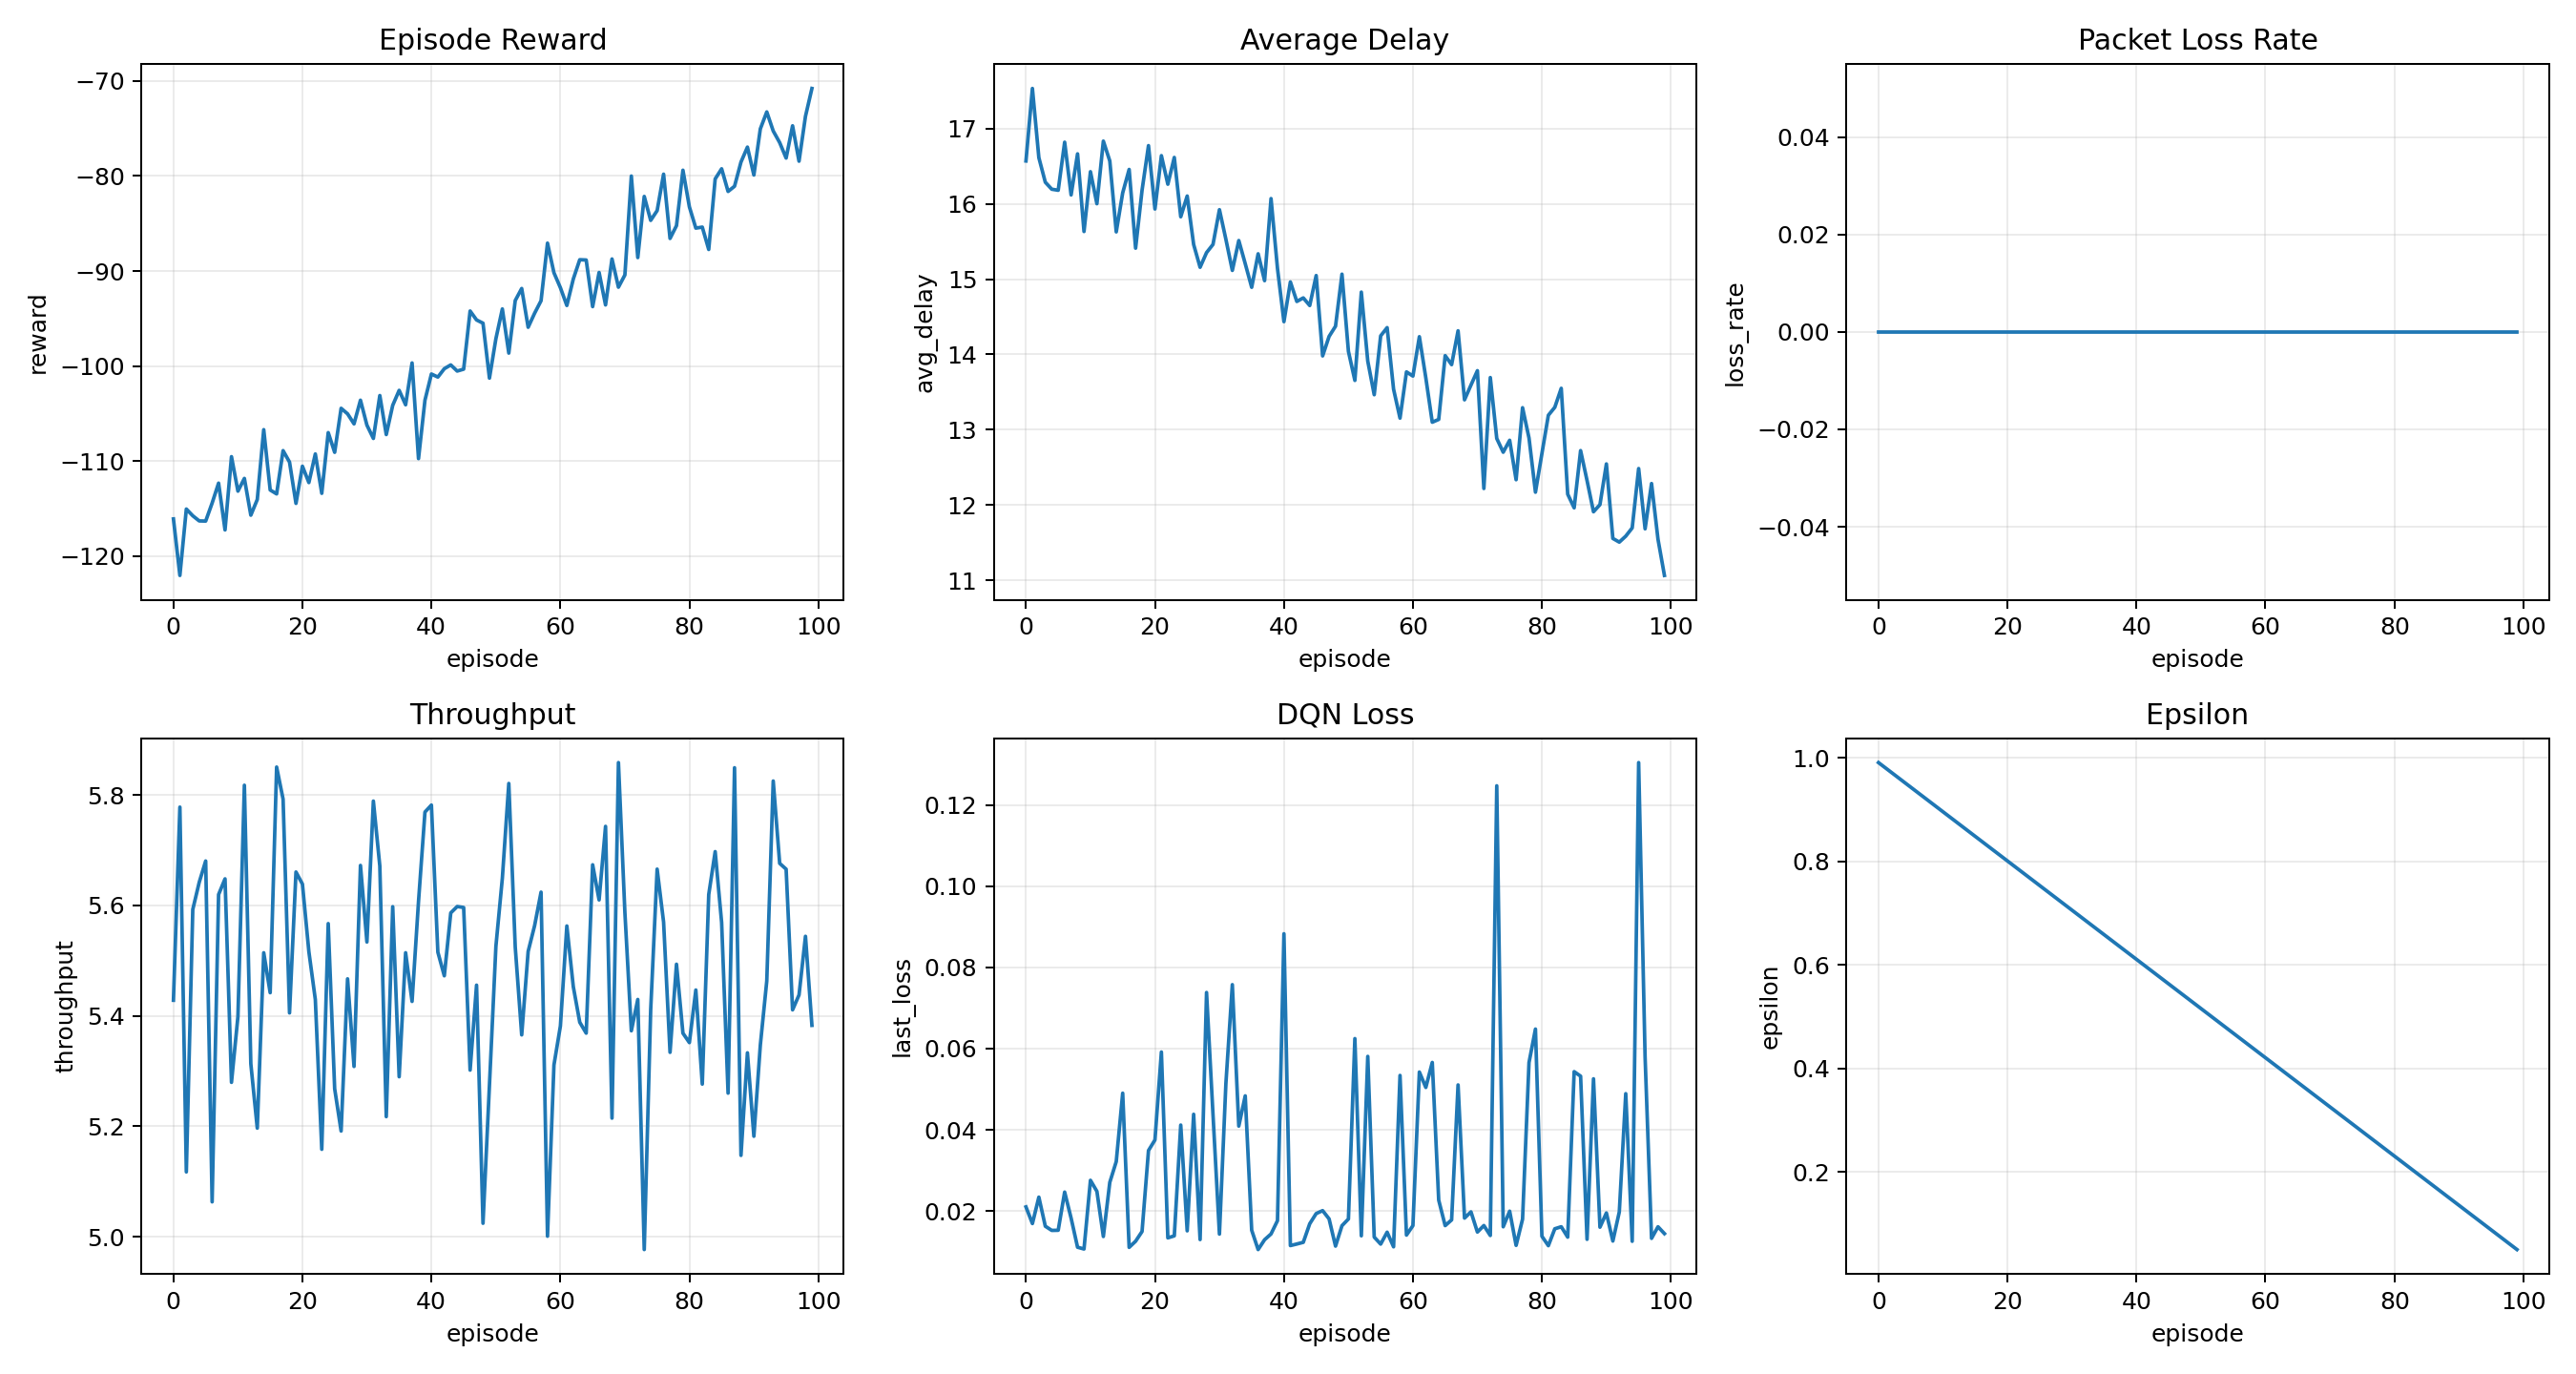
\includegraphics[width=0.92\textwidth]{figures/training_curves.png}
    \caption{Training curves for reward, average delay, packet loss rate, throughput, DQN loss, and epsilon.}
    \label{fig:en_training}
\end{figure*}

\begin{figure*}[t]
    \centering
    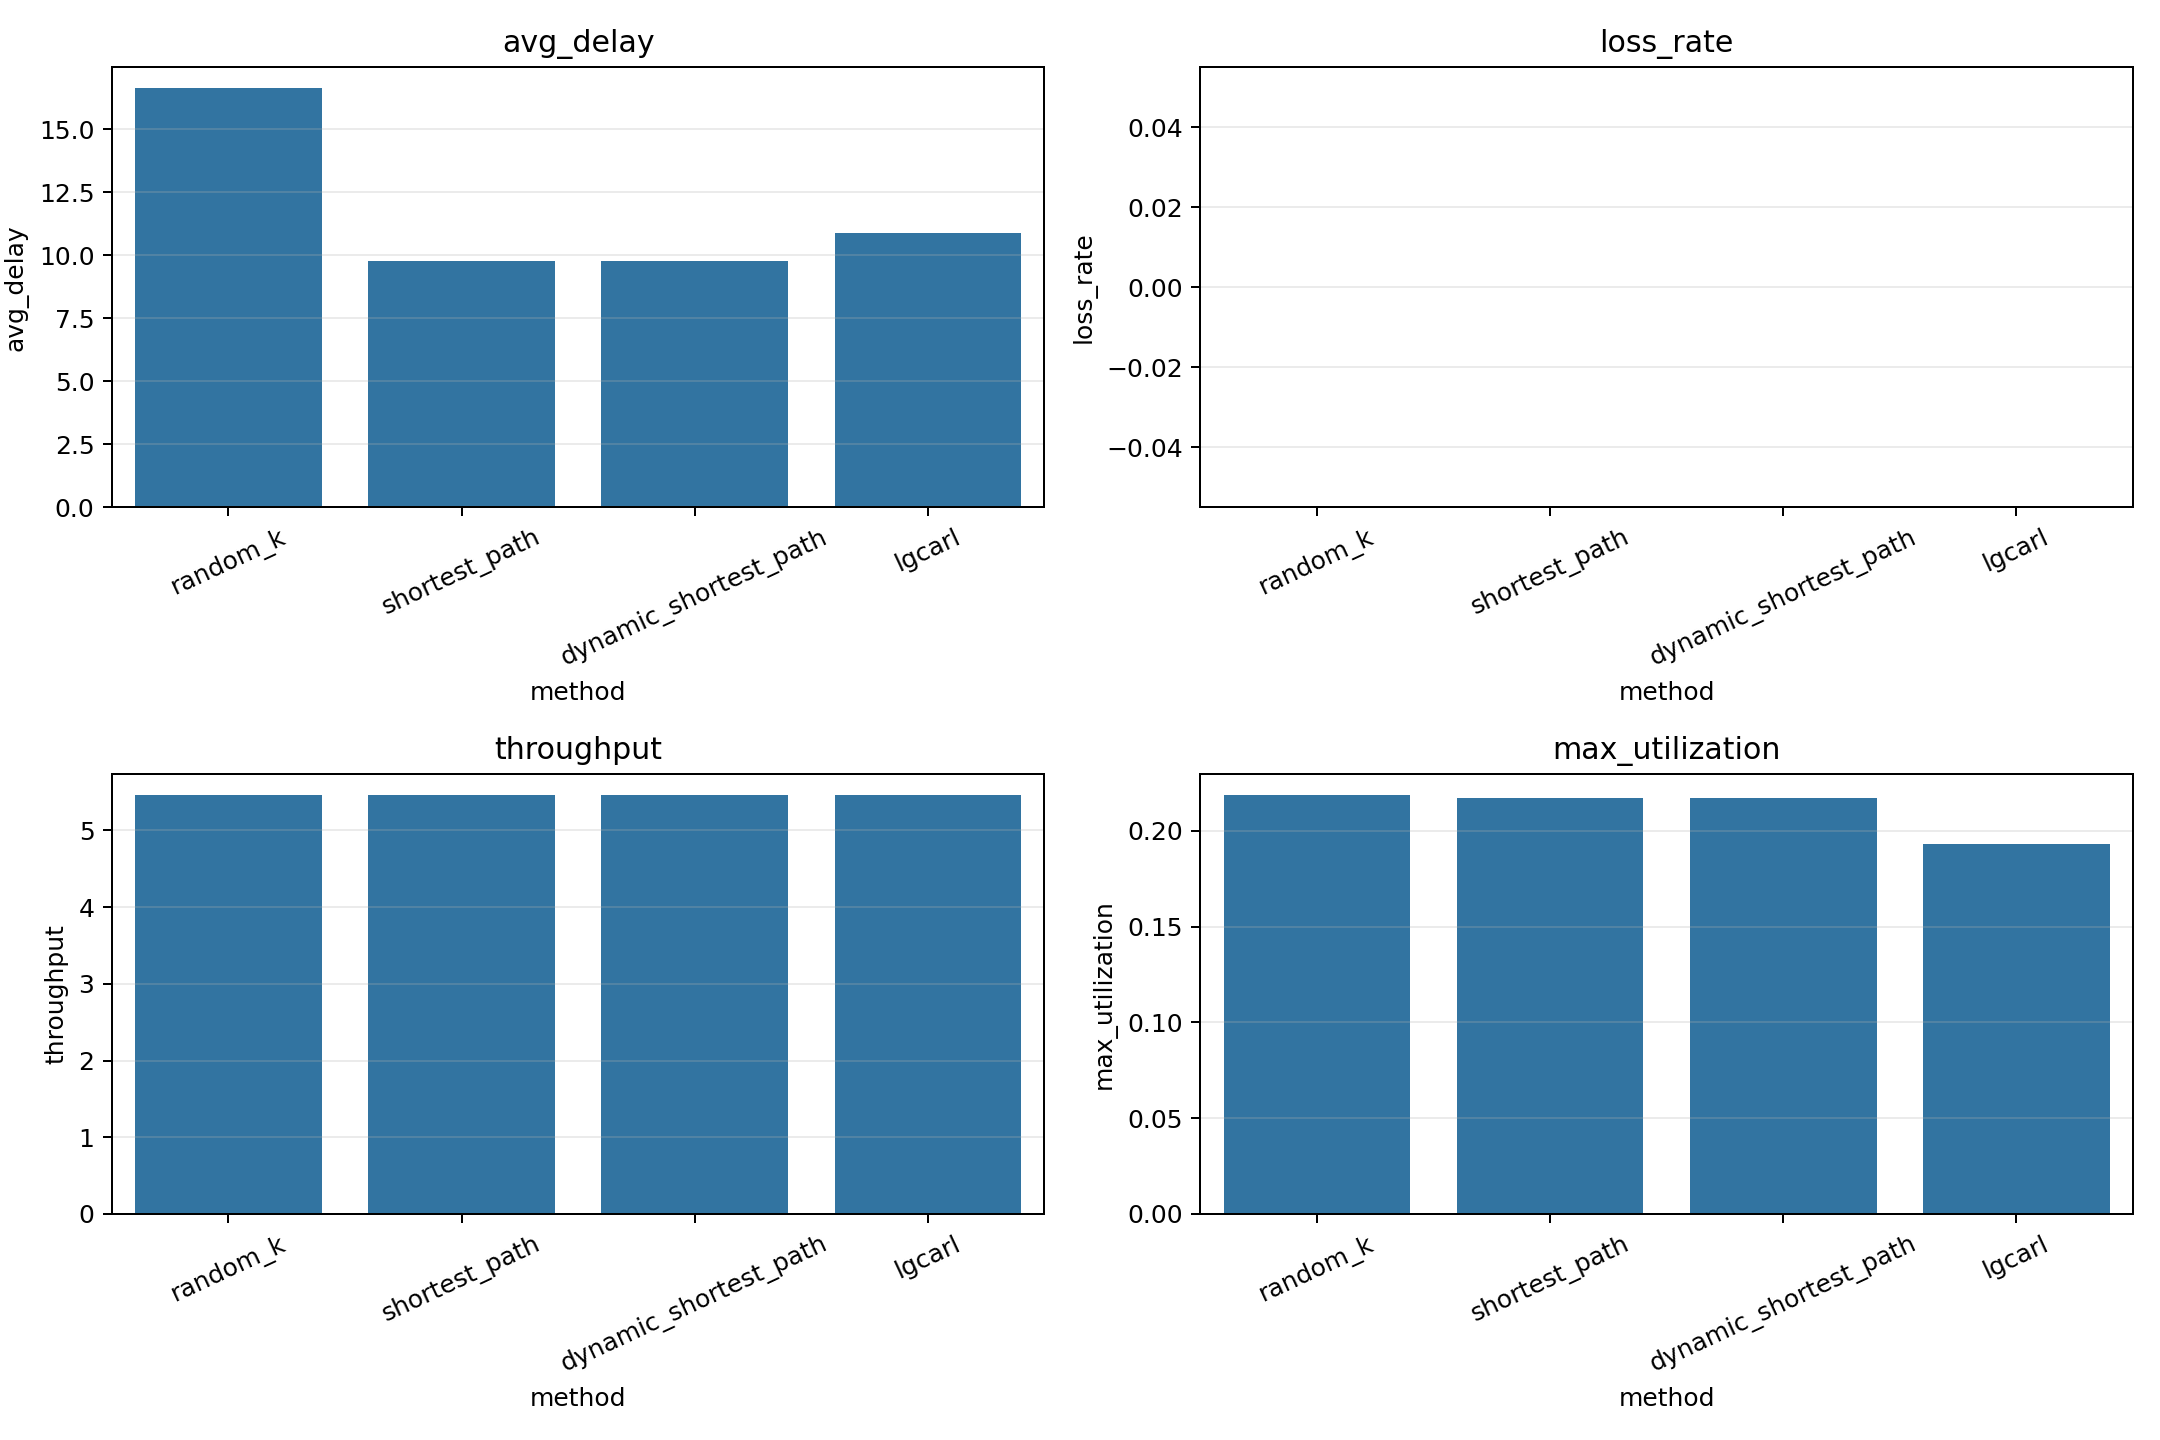
\includegraphics[width=0.92\textwidth]{figures/eval_bars.png}
    \caption{Evaluation bar charts comparing LG-CARL with routing baselines.}
    \label{fig:en_eval}
\end{figure*}

\section{Visualization Analysis}

To make the model behavior easier to interpret, the project implements route replay visualization. In the replay, nodes are routers and edges are network links. Warmer edges indicate higher link utilization, while the cyan highlighted route is the path selected by LG-CARL for the current flow. The right-side panel reports the current flow, demand, delay, loss, delivered traffic, and maximum utilization.

\begin{figure}[H]
    \centering
    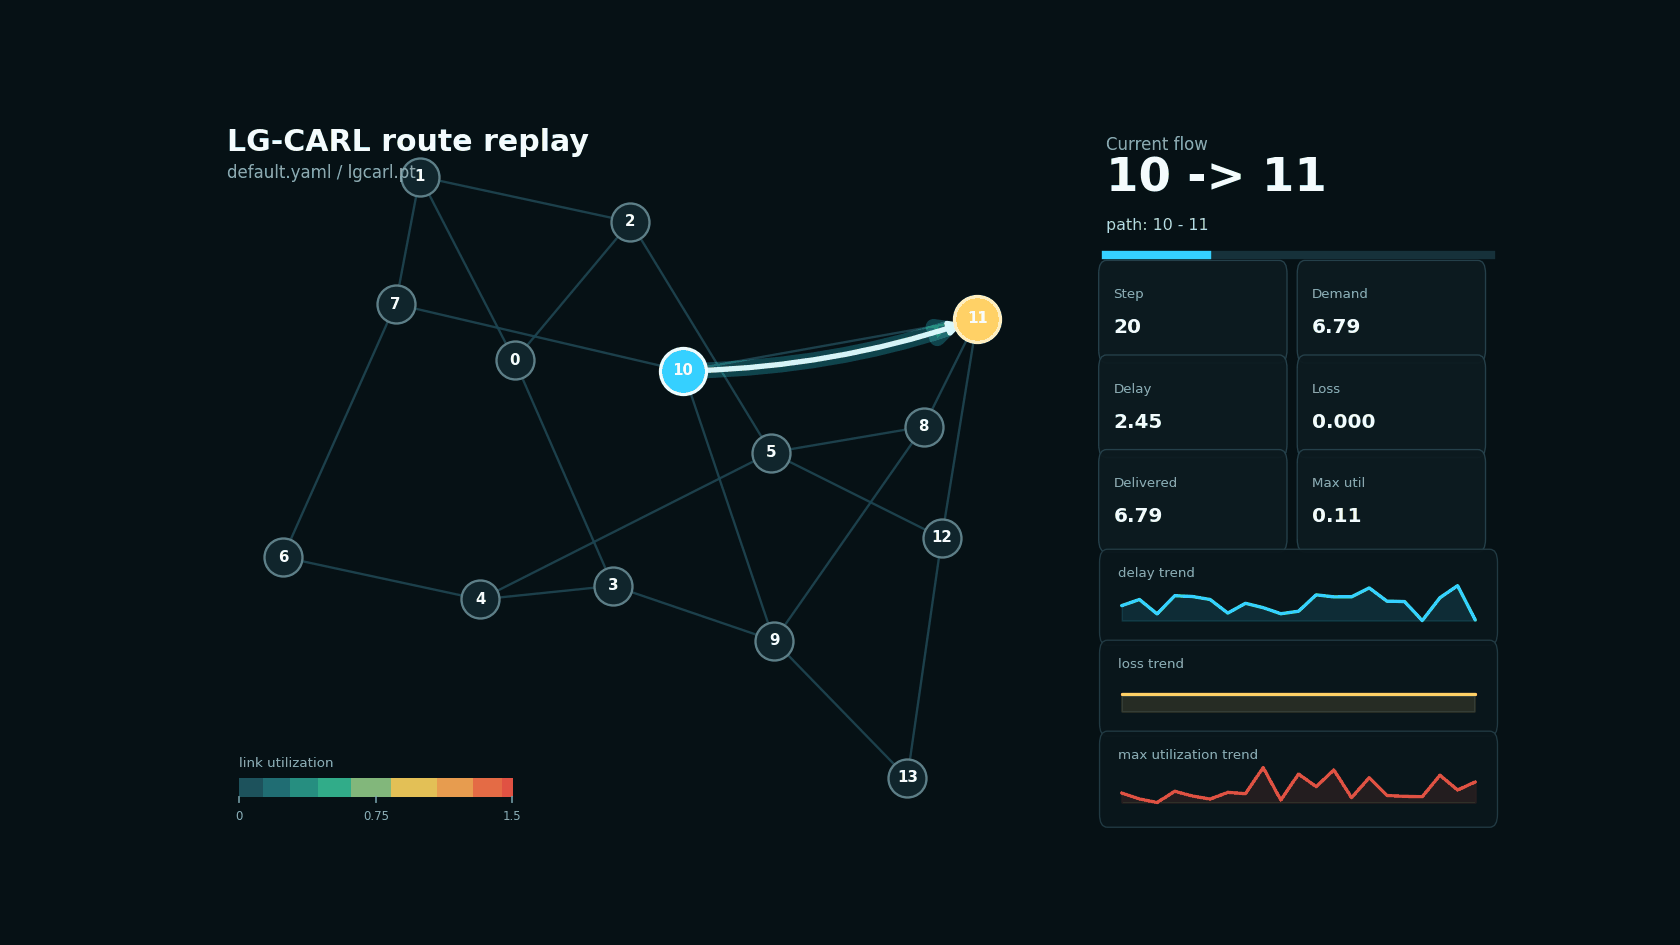
\includegraphics[width=0.98\columnwidth]{figures/route_replay_normal_frame.png}
    \caption{Route replay frame under regular traffic. The selected path is highlighted in cyan.}
    \label{fig:en_replay_regular}
\end{figure}

\begin{figure}[H]
    \centering
    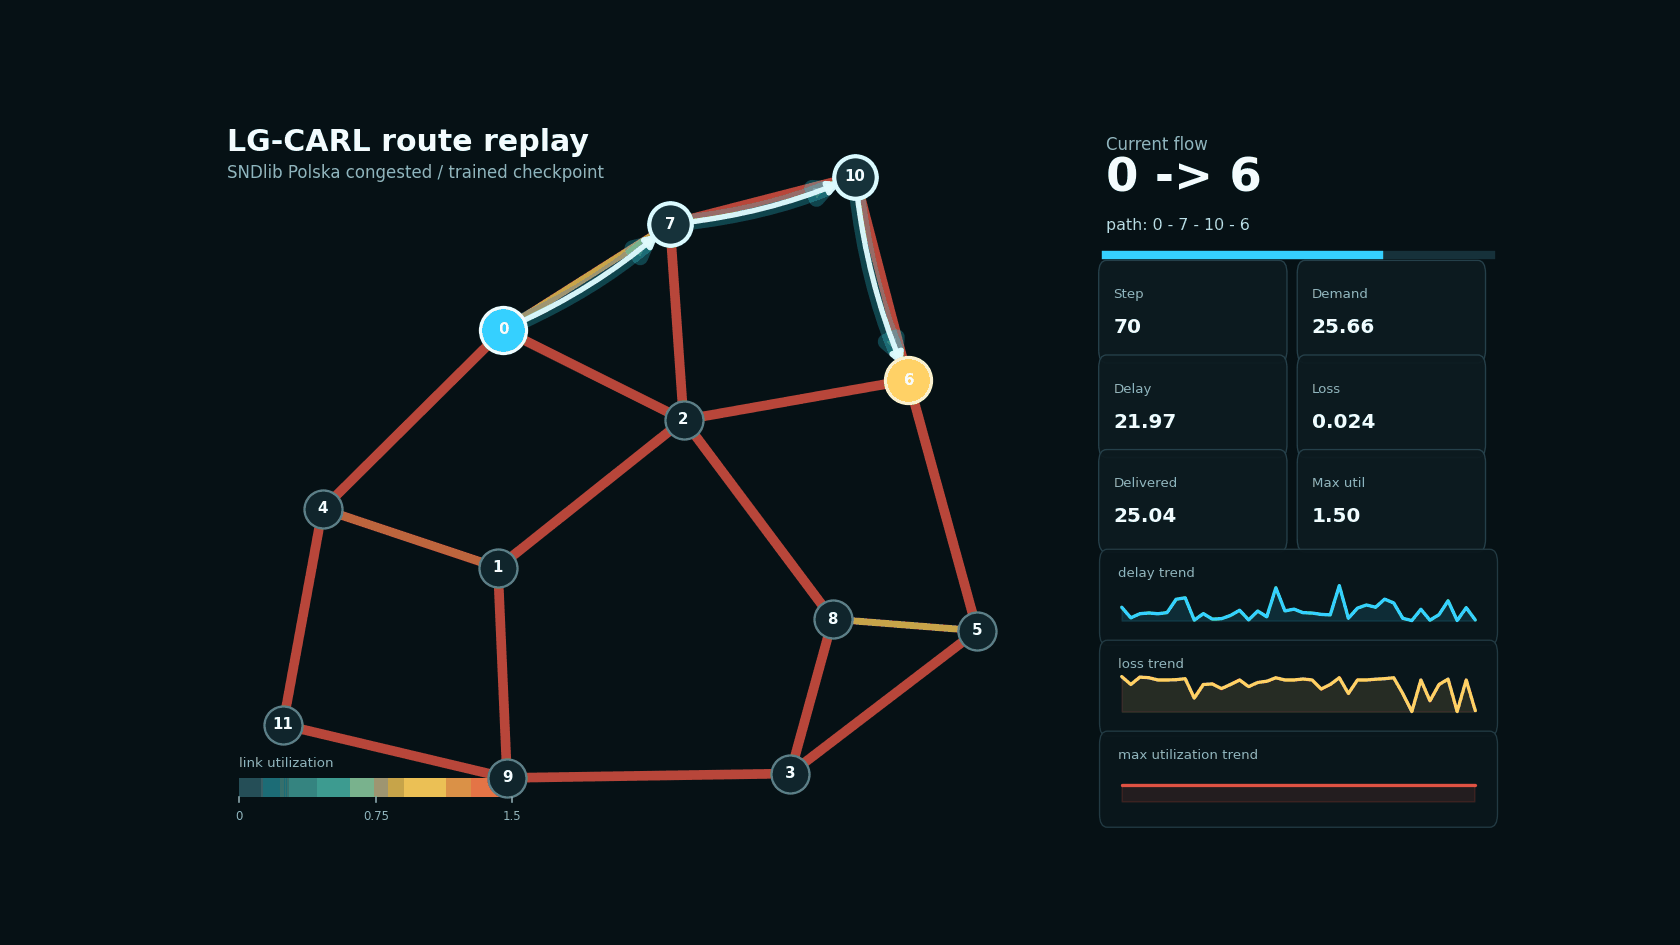
\includegraphics[width=0.98\columnwidth]{figures/route_replay_congested_frame.png}
    \caption{Route replay frame under heavy congestion. Many links become orange or red, and packet loss appears.}
    \label{fig:en_replay_congested}
\end{figure}

Under regular traffic, most links remain in cold colors and packet loss is nearly zero. Under congested traffic, multiple links reach high utilization, maximum utilization often saturates at 1.5, and the loss trend becomes visible. The GIFs are therefore useful for explaining policy behavior and network state changes. They should not be treated as standalone proof that the model outperforms a baseline; quantitative metrics such as those in \tabref{tab:en_results} remain the primary evidence.

\section{Conclusion}

This project implements a runnable GNN + RL adaptive routing system. LG-CARL encodes link-level state through a directed line graph and uses DQN to choose among candidate end-to-end paths. Under regular traffic, the learned policy reaches performance close to shortest-path and dynamic-shortest-path baselines. In some metrics, such as maximum link utilization and load balance, it shows a tendency to spread traffic more evenly.

However, the learned policy does not yet outperform dynamic shortest path under heavy congestion. The results show that LG-CARL learns load-balancing behavior, but this behavior is not sufficient to reduce packet loss or increase throughput in the most difficult setting. This suggests that reward weights, training stability, traffic distributions, and the reinforcement learning algorithm itself remain important areas for future improvement.

Overall, LG-CARL is a complete course-scale project. It includes a clear problem formulation, runnable implementation, multiple baselines, real-topology support, quantitative analysis, and interpretable visualizations. Future extensions could include reward ablation, double DQN, confidence intervals over multiple seeds, and generalization experiments on unseen topologies.

\section*{Acknowledgment}
\addcontentsline{toc}{section}{Acknowledgment}

The implementation and experiments were developed as a course project. The design is inspired by earlier work on Q-routing, graph neural network based network modeling, and deep reinforcement learning for control and routing \cite{boyan1993packet,rusek2020routenet,almasan2019deep,mnih2015human,hamilton2017inductive}.

\printbibliography

\end{document}
